% !TeX program = xelatex
%% 부득이하게 pdflatex을 사용해야 할 경우 위의 magic comment를 제거하십시오.

%%%%%%%%%%%%%%%%%%%%%%%%%%%%%%%%%%%%%%%%%%%%%%%%%%%%%%%%%%%%%%%%%%%%%%%%%%%%%%%%%
%%%  LaTeX document class of the thesis of the Gyeonggi Science High School   %%%
%%%  Last edition 2015.11.13 by Chinook Mok                                   %%%
%%%  Continously being modified by gshslatexintro after 2016.02.02.           %%%
%%%  Check the latest version at : latex.gs.hs.kr                             %%%
%%%  Also refer to https://www.facebook.com/gshstexsociety                    %%%
%%%%%%%%%%%%%%%%%%%%%%%%%%%%%%%%%%%%%%%%%%%%%%%%%%%%%%%%%%%%%%%%%%%%%%%%%%%%%%%%%

\documentclass{gshs_thesis}
\graphicspath{{images/}}
% 이곳에 필요한 별도의 패키지들을 적어넣으시오.
%\usepackage{...}
\usepackage{verbatim} % for commment, verbatim environment
\usepackage{spverbatim} % automatic linebreak verbatim environment
%\usepacakge{indentfirst}
\usepackage{tikz}
%\tikzset{
%	image label/.style={
%		every node/.style={
			%fill=black,
			%text=white,
%			font=\sffamily\scriptsize,
%			anchor=south west,
%			xshift=0,
%			yshift=0,
%			at={(0,0)}
%		}
%	}
%}
\usepackage{amsmath}
\usepackage{amsfonts}
\usepackage{amssymb}
\usepackage{float}
\usepackage{graphicx}
\usepackage{tabularx}
\usepackage{multirow}
\usepackage{booktabs}
\usepackage{longtable}
\usepackage{gensymb}
%\usepackage{subcaption}
%\usepackage{floatrow}
%\usepackage{pict2e}

\usepackage{pgfplots}
\pgfplotsset{
	compat=newest,
	label style={font=\sffamily\scriptsize},
	ticklabel style={font=\sffamily\scriptsize},
	legend style={font=\sffamily\tiny},
	major tick length=0.1cm,
	minor tick length=0.05cm,
	every x tick/.style={black},
}

\usetikzlibrary{shapes}
\usetikzlibrary{plotmarks}
\usepackage{listings}
\usepackage{hologo}
\usepackage{makecell}

\lstset{
	basicstyle=\small\ttfamily,
	columns=flexible,
	breaklines=true
}

\citation
\bibdata



% -----------------------------------------------------------------------
%                   이 부분은 수정하지 마시오.
% -----------------------------------------------------------------------
\titleheader{졸업논문청구논문}
\school{과학영재학교 경기과학고등학교}
\approval{위 논문은 과학영재학교 경기과학고등학교 졸업논문으로\\
졸업논문심사위원회에서 심사 통과하였음.}
\chairperson{심사위원장}
\examiner{심사위원}
\apprvsign{(인)}
\korabstract{초 록}
\koracknowledgement{감사의 글}
\korresearches{연 구 활 동}

%: ----------------------------------------------------------------------
%:                  논문 제목과 저자 이름을 입력하시오
% ----------------------------------------------------------------------
\title{Orion A Cloud의 쌍극 방출류의 성질} %한글 제목
\engtitle{Properties of Bipolar Outflows of the Orion A Cloud} %영문 제목
\korname{이 선 재} %저자 이름을 한글로 입력하시오 (글자 사이 띄어쓰기)
\engname{Lee, Seon Jae} %저자 이름을 영어로 입력하시오 (family name, personal name)
\chnname{李 善 在} %저자 이름을 한자로 입력하시오 (글자 사이 띄어쓰기)
\studid{16072} %학번을 입력하시오

%------------------------------------------------------------------------
%                  심사위원과 논문 승인 날짜를 입력하시오
%------------------------------------------------------------------------
\advisor{Park, Kie Hyun}  %지도교사 영문 이름 (family name, personal name)
\judgeone{박 용 선} %심사위원장
\judgetwo{강 동 일}   %심사위원1
\judgethree{박 기 현} %심사위원2(지도교사)
\degreeyear{2019}   %졸업 년도
\degreedate{2018}{7}{21} %논문 승인 날짜 양식

%------------------------------------------------------------------------
%                  논문제출 전 체크리스트를 확인하시오
%------------------------------------------------------------------------
\checklisttitle{[논문제출 전 체크리스트]} %수정하지 마시오
\checklistI{1. 이 논문은 내가 직접 연구하고 작성한 것이다.} %수정하지 마시오
% 이 항목이 사실이라면 다음 줄 앞에 "%"기호 삽입, 다다음 줄 앞의 "%"기호 제거하시오
%\checklistmarkI{$\square$}
\checklistmarkI{$\text{\rlap{$\checkmark$}}\square$}
\checklistII{2. 인용한 모든 자료(책, 논문, 인터넷자료 등)의 인용표시를 바르게 하였다.} %수정하지 마시오
% 이 항목이 사실이라면 다음 줄 앞에 "%"기호 삽입, 다다음 줄 앞의 "%"기호 제거하시오
%\checklistmarkII{$\square$}
\checklistmarkII{$\text{\rlap{$\checkmark$}}\square$}
\checklistIII{3. 인용한 자료의 표현이나 내용을 왜곡하지 않았다.} %수정하지마시오
% 이 항목이 사실이라면 다음 줄 앞에 "%"기호 삽입, 다다음 줄 앞의 "%"기호 제거하시오
%\checklistmarkIII{$\square$}
\checklistmarkIII{$\text{\rlap{$\checkmark$}}\square$}
\checklistIV{4. 정확한 출처제시 없이 다른 사람의 글이나 아이디어를 가져오지 않았다.} %수정하지 마시오
% 이 항목이 사실이라면 다음 줄 앞에 "%"기호 삽입, 다다음 줄 앞의 "%"기호 제거하시오
%\checklistmarkIV{$\square$}
\checklistmarkIV{$\text{\rlap{$\checkmark$}}\square$}
\checklistV{5. 논문 작성 중 도표나 데이터를 조작(위조 혹은 변조)하지 않았다.} %수정하지 마시오
% 이 항목이 사실이라면 다음 줄 앞에 "%"기호 삽입, 다다음 줄 앞의 "%"기호 제거하시오
%\checklistmarkV{$\square$}
\checklistmarkV{$\text{\rlap{$\checkmark$}}\square$}
\checklistVI{6. 다른 친구와 같은 내용의 논문을 제출하지 않았다.} %수정하지 마시오
% 이 항목이 사실이라면 다음 줄 앞에 "%"기호 삽입, 다다음 줄 앞의 "%"기호 제거하시오
%\checklistmarkVI{$\square$}
\checklistmarkVI{$\text{\rlap{$\checkmark$}}\square$} % usepackage 등의 명령어는 여기에.
\usepackage{cite}
\usepackage{tocloft}
\setlength{\cftbeforesecskip}{0pt}
\setlength{\cftbeforesubsecskip}{0pt}
\setlength{\cftbeforesubsubsecskip}{0pt}

\begin{document}
%	\renewcommand\baselinestretch{1.2} % line spacing in the paragraph

	\baselineskip=2.2em         % line spacing in the paragraph
	\maketitle  % command to print the title page with above variables
\setcounter{page}{1}
%---------------------------------------------------------------------
%                  영문 초록을 입력하시오
%---------------------------------------------------------------------
\begin{abstracts}     %this creates the heading for the abstract page
	\addcontentsline{toc}{section}{Abstract}  %%% TOC에 표시
	\noindent{
		Stars are born when matter from interstellar molecular clouds fall to its center to increase the mass of the protostar. Bipolar outflows are formed to remove the excess angular momentum of falling matter. Intensities of outflows are known as to be in a close relationship with their bolometric luminosity and evolutionary stages. In this study, data from Institute for Radio Astronomy in the Millimeter Range (IRAM) 30$\,$m Telescope and Taeduk Radio Astronomy Observatory (TRAO) were used. IRAM data were used to map $^{12}\textrm{CO}$ J = 2 - 1 over Orion A molecular cloud. TRAO data were used to map $^{13}\textrm{CO}$ J = 1 - 0 over the same region. Outflows were observed and measured by drawing contour maps and line profiles of  red/blue shifted components. The correlation between a protostar's luminosity and outflow momentum flux have been confirmed. Also, outflows could be detected better if the energy level of the emission line is higher. 
	}
\end{abstracts}

\begin{abstractskor}
	별은 성간분자운의 물질이 중심으로 떨어져 원시성의 질량을 증가시켜야만 탄생된다. 이 과정에서 중심으로 떨어지는 물질의 각운동량을 제거하기 위해 방출류가 발생한다. 여기서 방출류의 세기는 원시성의 진화 단계와 광도와 관련이 있다고 알려져 있다. 이를 새로 관측된 데이터를 사용하여 보다 좋은 방출류 측정 방법과 기존의 연구를 검증해 보려고 한다.이 연구에서는  Institute for Radio Astronomy in the Millimeter Range (IRAM) 30$\,$m 망원경으로 관측한 $^{12}$CO J = 2 - 1 관측 자료와 대덕 전파 망원경(Taeduk Radio Astronomy Observatory, TRAO)으로 관측한 $^{13}$CO J = 1 - 0 천이 선 자료를 이용하였다. 두 자료 모두 Orion A Cloud 영역을 담고 있다. 빠른 속도를 가진 적색/청색편이된 성분의 contour map을 그려 방출류를 관찰하고 방출류의 세기를 구하였다. 방출류의 세기와 원시성의 광도가 대체적으로 비례한다는 것을 알 수 있었다. 그리고 천이 선의 에너지 준위가 높을수록 방출류를 더 잘 검출할 수 있음을 확인할 수 있었다.
\end{abstractskor}
%----------------------------------------------
%   Table of Contents (자동 작성됨)
%----------------------------------------------
\cleardoublepage
\addcontentsline{toc}{section}{Contents}
\setcounter{secnumdepth}{3} % organisational level that receives a numbers
\setcounter{tocdepth}{3}    % print table of contents for level 3
\baselineskip=2.2em
\tableofcontents


%----------------------------------------------
%     List of Figures/Tables (자동 작성됨)
%----------------------------------------------
\cleardoublepage
\clearpage
\listoffigures	% 그림 목록과 캡션을 출력한다. 만약 논문에 그림이 없다면 이 줄의 맨 앞에 %기호를 넣어서 코멘트 처리한다.

\cleardoublepage
\clearpage
\listoftables  % 표 목록과 캡션을 출력한다. 만약 논문에 표가 없다면 이 줄의 맨 앞에 %기호를 넣어서 코멘트 처리한다.

%%%%%%%%%%%%%%%%%%%%%%%%%%%%%%%%%%%%%%%%%%%%%%%%%%%%%%%%%%%
%%%% Main Document %%%%%%%%%%%%%%%%%%%%%%%%%%%%%%%%%%%%%%%%
%%%%%%%%%%%%%%%%%%%%%%%%%%%%%%%%%%%%%%%%%%%%%%%%%%%%%%%%%%%
\cleardoublepage
\clearpage
\renewcommand{\thepage}{\arabic{page}}
\setcounter{page}{1}



 % Abstract

	%%%%%%%%%%%%%%%%%%%%%%%%%%%%%%%%%%%%%%%%%%%%%%%%%%%%%%%%%%%
	%%%% Main Document %%%%%%%%%%%%%%%%%%%%%%%%%%%%%%%%%%%%%%%%
	%%%%%%%%%%%%%%%%%%%%%%%%%%%%%%%%%%%%%%%%%%%%%%%%%%%%%%%%%%%
	% Next Section (e.g. Experiment, Linear theory, etc...) 
	% 이외에도 추가로 section마다 파일을 sub 폴더 안에 넣고 여기에서 
	% include 해주면 됩니다.
	% 예시 : methodology.tex을 sub 폴더안에 저장, 이 자리에 
	% \section{Obervations and Data Reduction}

\subsection{Observation Region}
The Orion region consists of two giant molecular clouds, the Orion A and B clouds. This study covers the Orion A Cloud. The Orion A Cloud covers about $29 \, \textrm{deg}^2$ of the sky and its distance is about 450$\,$pc \cite{kounkel2017gould}. The total mass is estimated to be about $10^5 \, M_{\odot}$. It contains several hot molecular cores, such as the BN-KL nebula. It is known that the Orion Cloud was formed by a collision and fragmentation between two giant molecular clouds about 60 million years ago. The effects of the collision can be seen at the present. There is a big velocity gradient along the declination axis. On the north side of the Orion A Cloud (OMC 2) shows about 12$\, \rm km\,s^{-1}$ but on the south end (L1641) it is about 5$\, \rm km\,s^{-1}$ \cite{schulz2012formation}.

\subsection{Observation Data}
%%% 박기현 수정 시작
The $^{12}\textrm{CO (J = 2 - 1, 230.538\,GHz)}$ data was observed with the IRAM $\textrm{30\,m}$ telescope in Granada, Spain, in 2013. The spatial beamwidth was $\textrm 11^{\prime\prime}$, and the spectral resolution was 0.4$\, \rm km\,s^{-1}$. The noise level was 0.2$\, \rm K$. It only covers the north region of the Orion A cloud \cite{berne2014iram}.

The $^{12}\textrm{CO (J = 1 - 0, 115.271\,GHz})$ data was observed with the NRO 45m telescope in Nobeyama, Japan.

The $^{13}\textrm{CO (J = 1 - 0, 110.201\,GHz})$ and the $\textrm{C}^{18}\textrm{O (J = 1 - 0, 109.782\,GHz})$ data were observed with the $\textrm{13.7\,m}$ telescope at Taeduk Radio Astronomy Observatory (TRAO) in 2017. The spatial beamwidth was $\textrm 45^{\prime\prime}$, and the spectral resolution was 0.05$\, \rm km\,s^{-1}$. The noise level was 0.4$\,$K.
$^{13}\textrm{CO}$ and $\textrm{C}^{18}\textrm{O}$ lines are optically thin lines which can trace most of the matter on the line of sight, contrasting to $^{12}\textrm{CO}$ lines which are so optically oblique that it can only trace the outermost part of the molecular core. In this study, I used TRAO data to determine the protostar's velocity and linewidth which are the kinematic properties of the envelope. Then, I will trace the outflow jets using $^{12}$CO data.
%%%박기현 수정 끝

%%%선재 원본
%%%The $^{12}$CO(J = 2 - 1, $230.538\,\rm GHz$) data was observed with the IRAM 30$\,$m telescope in Granada, Spain, in 2013. The spatial beamwidth was 11", and the spectral resolution was 0.4$\, \rm km\,s^{-1}$. The noise level was 0.2$\, \rm K$. It only covers the north region of the Orion A cloud \cite{berne2014iram}. \\
%%%The $^{12}$CO (J = 1 - 0, $115.271\, \rm GHz$) data was observed with the NRO 45m telescope in Nobeyama, Japan.  \\
%%%The $^{13}$CO (J = 1 - 0, $110.201\,$GHz) and the $\textrm{C}^{18}\textrm{O}$(J = 1 - 0, 109.782 GHz) was observed at Taeduk Radio Astronomy Observatory (TRAO) 13.7$\,$m telescope in 2017. The spatial beamwidth was 45", and the spectral resolution was 0.05$\, \rm km\,s^{-1}$. The noise level was 0.4$\,$K.\\
%%%$^{13}$CO and $\textrm{C}^{18}\textrm{O}$ lines are optically thin lines which can trace most of the matter on the line of sight, contrasting to $^{12}$CO lines which are so optically oblique that it can only trace the outermost part of the molecular core. In this study, I used TRAO data to determine the protostar's velocity and linewidth which are the kinematic properties of the envelope. Then, I will trace the outflow jets using $^{12}$CO data.

Figure \ref{fig:map1} shows the data from IRAM and TRAO. The intensity of the $^{12}\textrm{CO}$ data is approximately 10 times stronger than the $^{13}\textrm{CO}$ data.

%\begin{figure}[h]
\begin{figure}[t]
	\begin{center}
		\begin{tabular}{cc}
			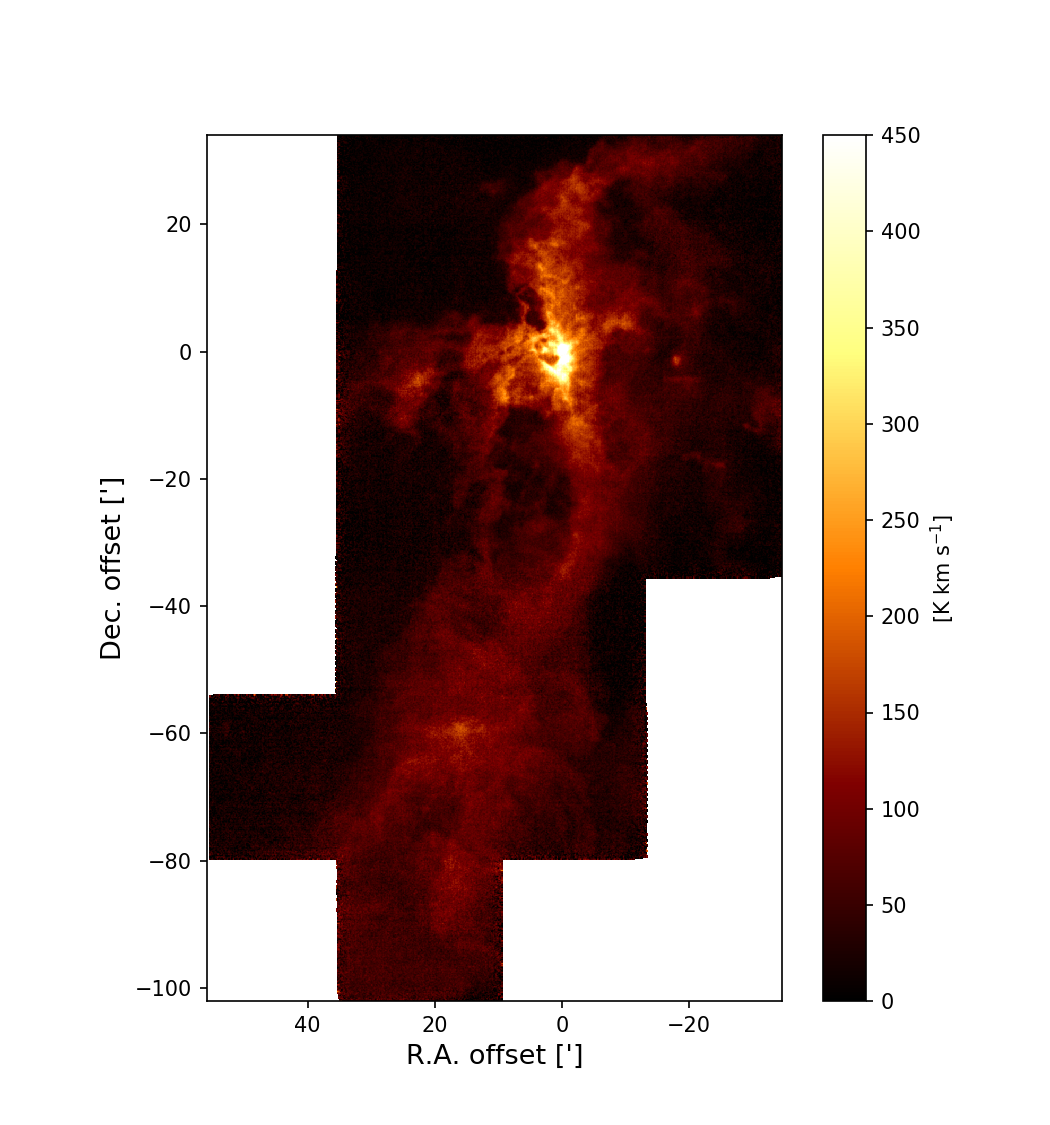
\includegraphics[width=0.45\textwidth]{RNE_12CO_Orion} & 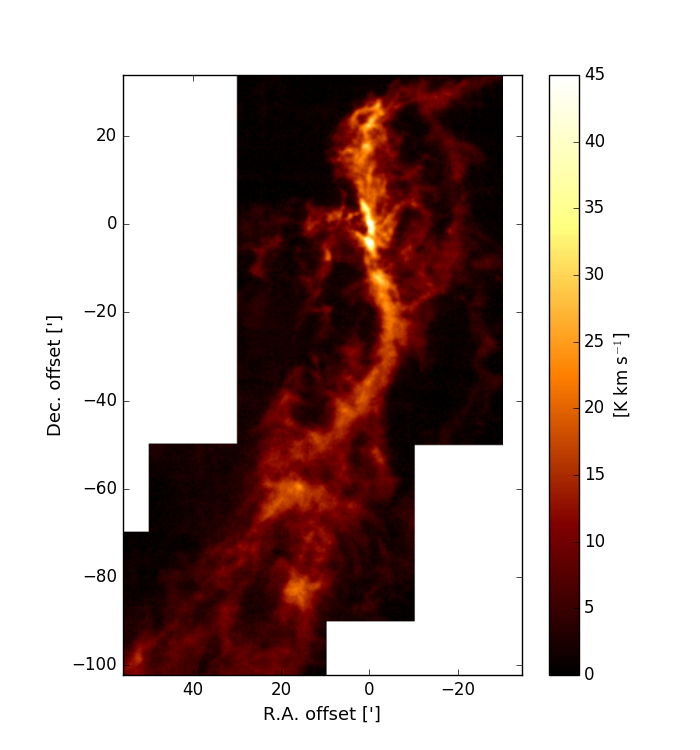
\includegraphics[width=0.45\textwidth]{Orion_13CO_intmap}
		\end{tabular}
	\end{center}
	\caption{Orion A $^{12}$CO (J = 2 - 1) integrated intensity map (left) $^{13}$CO (J = 1 - 0) integrated intensity map (right).}
	\label{fig:map1}  %%%박기현샘 추가함 (이렇게 넣어야 제데로 ref 됨.)
	%%% 박기현 레이블을 달고, 본문에서 언급하면 latex에서 알아서 같은 페이지로 보내줌.
\end{figure}

\subsection{Identification of Outflows}
Data obtained by observing radio waves were summed over the line of sight, which tells us the distribution of matter which has relative radial velocity to the observer. The envelope around the protostar is static or is contracting slowly to the protostar itself, but outflow jets have large velocity components from each pole. If the inclination of the outflows are not zero, it would be seen as jets are moving closer or further from the observer. 
In this study, $^{13}$CO and $\textrm{C}^{18}\textrm{O}$ lines were used to get the velocity distribution of the protostar. By using Gaussian fitting, I calculated the protostar’s central velocity($v_{cen}$) and the full width at half maximum (FWHM). The intervals of the red/blue lobes were defined by how far they were from the center velocity and how strong the intensity is.

Because the emission lines of $^{12}$CO are optically thicker than other lines, it is appropriate to trace the outflows with $^{12}$CO lines. I drew contour maps to find out if bipolar outflows existed with the protostar at its center. To check if the red/blue lobes that are found are outflows from the same protostar I checked the $^{12}$CO, $^{13}$CO, $\textrm{C}^{18}\textrm{O}$ lines from the red peak, blue peak, and the center points. For each outflow confirmed, I calculated the column density and the momentum force.

The column density can be calculated as the following expression:
\begin{align}
	N_{H_2} =& \frac{8\pi \nu^3}{c^3} \frac{1}{(2J_l +3)A}  \notag \\
	& \times \frac{Z(T_{ex})}{exp(-E_l / kT_{ex})[1-exp(h\nu / kT_{ex})]} \notag \\
	& \times \frac{\int T_B dV}{J(T_{ex})-J(T_{bg})} \label{column_density}
\end{align}

\begin{equation}
J(T) = \frac{h \nu / k}{exp(h\nu / kT)-1}
\end{equation}

In equation (\ref{column_density}), $\nu$ is the corresponding frequency of emission line, $c$ is the speed of light, $J_l$ is the rotational quantum number of the lower energy level, $A$ is the Einstein A coefficient, $Z$ is the partition function, $E_l$ is the rotational energy of the lower energy level, $k$ is the Boltzmann's constant, $T_{ex}$ is the excitation temperature of the transitions, $\int T_B dV$ is the integrated intensity measured, and $T_{bg}$ is the background radiation temperature. I assumed a local thermal equilibrium(LTE) excitation at an outflow temperature of 50$\,$K \cite{takahashi2008millimeter}.
The mass within one beam can be calculated as the following:

\begin{equation}
M_B =  \frac{\pi}{4} D^2 \theta_B ^2 X[\textrm{CO}] N_{\textrm{H}_2} m_{\textrm{H}_2} \label{beam_mass}
\end{equation}

$D$ is the distance to the objects, $\theta_B$ is the beam size, and $m_{\textrm{H}_2}$ is the mass of one hydrogen molecule. $X[\textrm{CO}]$ is the abundance ratio of CO to $\textrm{H}_2$. In this paper, $D = 450\,\textrm{pc}$ and $X[\textrm{CO}] = 10^{-4}$ was used \cite{hatchell2007star}.\\

\subsection{Calculating Momentum Flux}

The momentum flux within one beam is calculated as the following:

\begin{equation}
\dot{P} = \frac{dP}{dt} = \sum_{v} {\frac{M_B (v) (v/ \cos i)}{D\theta_B / (v \tan i)}}
\end{equation}

$v$ is the velocity offset from $v_{cen}$, $M_B (v)$ is the mass within one beam, and $i$ is the inclination within one beam \cite{hatchell2007star}.
Then the momentum flux from individual beams were summed in annuli. 

\begin{equation}
F_{\textrm{CO}} = \sum _{annulus} \frac{2\pi \theta_r}{N_{pix}\theta_B}\dot{P}	
\end{equation}

$N_{pix}$ is the number of pixels in a annulus. $\theta_r$ is the distance between each pixel and the outflow center. $\theta_B$ is the beam size \cite{hatchell2007star, van2013outflow}.
 와 같이 작성
	%%%% 주의
	%%%% 파일이 나뉠 때마다 자동으로 페이지넘김(\clearpage)가 됩니다. 
	%%%% 따라서 subsection을 나누는 용도로는 사용하지 마십시오.
	%%%% \include{sub/experiment} 와 같이...
	
	
\section{Introduction}

별들은 분자운에서 중력 수축을 통해 태어난다. 별 탄생 초기 단계에서 어린 원시성(young stellar objects; YSOs)들은 아직 분자운 속에서 묻혀 있으며, 원시성 주변 성간 물질을 중력적으로 끌어들이며 원시성의 질량과 온도를 증가시킨다. 원시성으로 물질이 유입되는 과정에서 각운동량이 보존되기 때문에 별 주변에서는 물질이 매우 빠르게 물질이 회전하고, 물질이 더 이상 별로 들어가기 힘들어진다. 그러나 별 생성 과정에서 각운동량을 제트나 쌍극방출류(bipolar outflows)로 제거하기 때문에, 관측적으로 원시성에 유입되는 물질의 양과 비례하는 방출류가 발생한다. \cite{Bontemps} \\
원시성에 유입되는 물질의 양과 원시성의 광도가 비례한다는 사실은 이미 알려져 있다. \cite{Kang} 방출류의 세기(outflow force)는 원시성들이 Class 0에서 Class I으로 진화할수록 감소하고, 이것은 원시성이 성간 물질을 끌어당기는 정도가 줄어든다는 것을 알려준다. \\
별 탄생의 초기 단계는 두꺼운 외피로 둘러쌓여 있어서 중심 원시성으로의 물질 유입을 직접적으로 관측하기는 힘들다. 앞서 언급한 방출류에 대해 지금까지 연구된 특성은 원시성으로의 물질 유입에 대해 간접적인 연구를 가능하게 한다. 다양한 원시성에서 나오는 방출류에 대해서는 지금까지 많은 연구가 되어 있다.\\
본 연구에서는 Orion A Cloud와 ρ Ophichus Cloud 안에 있는 원시성들과 그 방출류를 관찰하려고 한다. Orion A Cloud은 Spitzer 망원경 \cite{Spitzer} \cite{OphDunham} 과 Herschel \cite{HerschelFurlan} 원시성 catalogue를 참고하여 방출류를 관측할 수 있는 원시성들을 선택한 후, NRO $^{12}CO$ 관측 데이터와 TRAO $^{13}CO$, $C^{18}O$ 관측 데이터를 이용해서 기원 원시성들의 알려진 방출류를 분석하여 방출류의 세기와 복사 광도의 비례 관계를 다시 확인해보자 한다. 또한 복사 온도와 SED의 기울기를 통해 원시성의 진화단계를 확인하고, 방출류의 세기와의 관계를 찾아보려고 한다. \\
이 연구를 위해서는 우선 천문학 자료를 이해하기 위한 기초 지식이 필요하다. 그래서 2장 이론적 배경에서는 복사전달 방정식과 아인슈타인 계수와 관계식으로부터 설명을 시작하여 기둥 밀도와 방출류의 세기를 구하는 식까지 나타내었다. 2장의 나머지 부분에서는 본 연구에서 관측하고자 하는 대상과 지금까지 받아들여지고 있는 원시성의 진화 단계와 방출류에 대해 정리하였다. 3장은 본 연구에서 사용한 관측 데이터에 대해 나타내었다. 4장은 분석으로 관측 데이터로부터 contour map을 그려 방출류를 검출하고 방출류의 세기를 측정하는 과정과 SED를 그린 과정을 정리하였다. 5장은 결과로 관측한 원시성들에 대한 정보와 방출류가 검출된 contour map과 line profile, SED를 나열하였다. 6장 토의는 알아낸 결과들을 기존 연구와 비교하여 다양한 변인들과 방출류의 세기와의 관계를 분석해보았다. 7장은 결론 및 제언으로 결과와 토의들로 얻어낸 결론과 추후 연구에 추가하면 좋을 점들을 정리하였다.



%-----------------------------------------------------
% Next Section (e.g. Experiment, Linear theory, etc...) 
%-----------------------------------------------------
\section{이론적 배경}

\subsection{복사전달 방정식}
멀리 떨어져 있는 천체로부터 오는 빛을 보면 그 천체에서 일어나는 현상을 알 수 있다. 빛은 천체 현상이 일어난 곳의 물질과 상호 작용하여 성질이 바뀌게 되는데 이를 기술하는 것이 '복사전달 방정식'이다.\\
빛, 즉 복사장을 기술하는 물리량 중 실험적으로 측정 가능하고 가장 기본적인 것으로는 플럭스가 있다. 플럭스 (Flux, $F_\nu$)는 단위 시간동안 단위 면적을 통과하는 특정 주파수의 빛의 에너지로 단위는 [erg s$^{-1}$ cm$^{-2}$ Hz$^{-1}$]이다. 플럭스보다 엄밀하게 복사장을 기술하기 위해 빛의 세기(Intensity, $I_\nu$)를 사용한다. 이는 주어진 방향에서 단위 입체각에서 들어오는 단위 면적당 단위 시간당 특정 주파수에서의 에너지이다.	빛의 세기의 단위는 [W m$^{-2}$ sr$^{-1}$ Hz$^{-1}$]이고, 플럭스와는 다르게 거리와 무관하다는 특징을 갖고있다.\\
빛이 물질을 통과하여 지나갈 때 물질로부터 빛이 방출되어 빛의 세기가 강해지기도 하고 흡수되어 약해지기도 한다. 미소 길이 $ds$ 를 지날 때 방출되는 특정 주파수에서의 빛의 세기를 $dI_{\nu} ^{+} = j_{\nu} ds$ 라고 하자. 흡수되는 빛의 세기를 $dI_{\nu} ^{-} = \kappa_{\nu} I_{\nu}ds$라고 하자. $j_{\nu}$는 방출 계수이고 $\kappa_{\nu}$는 흡수 계수이다. 빛의 주파수에 따라서 Intensity와 흡수, 방출 정도가 달라지기 때문에 논의하는 대부분의 변수들이 모두 $\nu$의 함수로 나타내어진다. \\
이것을 이용해 복사전달 방정식을 다음과 같이 표현할 수 있다. 
\begin{equation}
dI_\nu = j_{\nu}ds - \kappa_{\nu} I_{\nu}ds
\end{equation}
\begin{equation}
\frac{dI_\nu}{ds} = j_{\nu} - \kappa_{\nu} I_{\nu}
\end{equation}
성간 물질의 개수 밀도가 $n$/cm$^3$라고 할 때, 각 입자가 빛을 흡수하는 유효 단면적을 $\sigma _\nu$라고 하자. $\kappa_\nu = n \sigma _\nu$라는 관계가 성립한다.\\
광학적 깊이 $\tau_\nu$ (optical depth)를 다음과 같이 정의하자. 
\begin{equation}
d\tau_\nu = -\kappa _\nu ds
\end{equation}
여기에서 $-$ 부호는 빛이 나아가는 방향과 반대로 관측자로부터 얼마나 떨어졌는지를 측정한다는 것을 의미한다.\\
Source function($S_\nu$) 를 다음과 같이 정의하자.
\begin{equation}
S_\nu = \frac{j_\nu}{\kappa_\nu}
\end{equation}
복사전달 방정식을 다음과 같이 쓸 수 있다. 
\begin{equation}
\frac{dI_\nu}{d\tau_\nu} = I_\nu - S_\nu \label{RT}
\end{equation}
복사전달 방정식의 일반해를 구해보자. \\
$(\ref{RT})$ 의 양변에 $e^{-\tau_\nu}$를 곱하고, 우변의 첫번째 항을 좌변으로 옮기자.
\begin{equation*}
	\frac{dI_\nu}{d\tau_\nu} e^{-\tau_\nu} - I_\nu e^{-\tau_\nu} = - S_\nu e^{-\tau_\nu}
\end{equation*}
좌변을 다음과 같이 바꿀 수 있다. 
\begin{equation*}
	\frac{d \left(I_\nu e^{-\tau_\nu}\right)}{d\tau_\nu} = - S_\nu e^{-\tau_\nu}
\end{equation*}
양변을 $\tau_\nu$에 대하여 적분하면 다음과 같이 정리할 수 있다. 여기서 $I^0$는 입사하는 빛의 세기이다.
\begin{equation*}
	I_\nu = I_\nu ^0 e^{-\tau_\nu} + \int_{0}^{\tau_\nu} S_\nu e^{-t}dt
\end{equation*}
$S_\nu$가 성간운 전체에 대하여 일정하다면 다음과 같이 표현된다.
\begin{equation}
I_\nu = I_\nu ^0 e^{-\tau_\nu} + S_\nu \left(1-e^{-\tau_\nu}\right) \label{RTsol}
\end{equation}
성간운이 optically thin한 상태라면 $e^{-\tau_\nu}\approx 1-\tau_\nu$로 근사할 수 있고, $(\ref{RTsol})$을 $I_\nu = I_\nu ^0 + \left(S_\nu - I_\nu ^0\right) \tau_\nu$로 쓸 수 있다. 여기서 $S > I^0$이면 방출선이고 $S < I^0$이면 흡수선이다.\\


\subsection{아인슈타인 계수와 관계식}

\begin{figure}[h]
	\begin{center}
		\begin{tabular}{ccc}
			\centering
			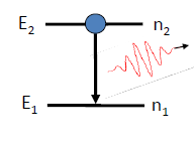
\includegraphics[width=4.5cm]{Einstein1.png} & 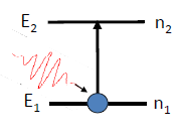
\includegraphics[width=4.5cm]{Einstein2.png} & 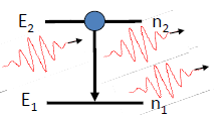
\includegraphics[width=6cm]{Einstein3.png}\\
			(a) 자발적 광자 방출 & (b) 광자 흡수 & (c) 유도 방출\\[6pt]
		\end{tabular}
	\end{center}
	\caption{전자와 광자의 상호작용}
\end{figure}

아인슈타인은 흡수계수와 방출계수를 미시적 관점에서 보았다. 성간운에서 빛이 흡수되거나 방출되는 방법에는 세 가지 방법이 있다. 첫번째 방법은 자발적 방출이다. 전자가 한 에너지 준위에서 다른 에너지 준위로 자발적으로 떨어지면서 광자를 방출하는 것이다. 레벨 2가 레벨 1보다 $h\nu_0$만큼 에너지가 높은 준위라고 할 때, 레벨 2에서 레벨 1으로 전자 천이가 벌어질 확률을 $A_{21}$이라고 하자.\\
두 번째 방법은 전자가 광자를 흡수해서 레벨 1에서 레벨 2로 올라가는 것이다. 이럴 때 흡수선이 생긴다. 
이상적으로는 방출선이나 흡수선이 생길 때 정확하게 하나의 주파수에서만 빛이 검출되어야 한다. 하지만 기체의 온도로 인하여 전자가 에너지를 가지게 되고, 불확정성 원리에 의해 전자의 속도가 정확하게 정해지지 않는다. 속도를 가지고 있는 입자에서 나온 빛은 도플러 효과에 의해 주파수가 바뀌게 된다. 이것을 line profile 이라고 부르고, 특정 주파수 $\nu_0$를 중심으로 넓게 퍼지게 된다. 이론적으로는 gaussian distribution을 따르게 되고, 이 함수를 $\phi(\nu)$라고 한다. $\int_{0}^{\infty}\phi(\nu)d\nu = 1$이 되도록 정의한다. 그리고 모든 방향에서들어오는 모든 빛의 세기의 평균값을 평균세기(mean intensity)라 하고 $J_\nu=\int I_\nu(\Omega) d\Omega$로 정의한다. $\bar{J} = \int_{0}^{\infty}J_\nu\phi(\nu)d\nu$로 정의하여 $B_{12}\bar{J}$를 레벨 2에서 레벨 1으로 전자 천이가 벌어질 확률이라고 하자.\\
또한 원자 주변에 복사장이 있으면 지나가는 광자에 의해 전자가 레벨 2에서 레벨 1으로 떨어지게 할 수 있다. 이 세 번째 방법은 유도 방출으로 일어날 확률을 $B_{21} \bar{J}$라고 하자.\\
열역학적 평형 상태에 있는 경우, 미시적 평형이 이루어져야 한다. 즉, 레벨 2에서 1으로 떨어지면서 광자를 방출하는 전자의 수와 광자를 흡수하며 레벨 1에서 2로 올라가는 전자의 수가 같아야 한다. $n_1$을 레벨 1에 있는 전자의 밀도, $n_2$를 레벨 2에 있는 전자의 밀도라고 하면 다음 식이 성립한다.
\begin{equation}
n_1 B_{12} \bar{J} = n_2 A_{21} + n_2 B_{21} \bar{J}
\end{equation}

이 식을 정리하면 다음과 같이 된다. 
\begin{equation}
\bar{J} = \frac{\frac{A_{21}}{B_{21}}}{\frac{n_1}{n_2}\frac{B_{12}}{B_{21}}-1}
\end{equation}
열역학적 평형상태이므로 각 준위에 있는 전자의 밀도는 볼츠만 방정식을 따르고 ($n_2/n_2 = g_2/g_1$ exp($-h\nu/kT$)), 식은 다음과 같이 정리된다. 
\begin{equation}
\bar{J} = \frac{\frac{A_{21}}{B_{21}}}{\frac{g_1 B_{12}}{g_2 B_{21}}e^{\frac{h \nu_0}{kT}}-1} \label{Jbar-1}
\end{equation}
열역학적 평형 상태에서 복사장은 흑체 복사를 하게 되므로 복사장의 세기는 플랑크 함수로 표현되고, 
\begin{equation}
\bar{J} \approx B_\nu (\nu_0) = \frac{2h\nu_0^3}{c^2} \frac{1}{e^{\frac{h\nu_0}{kT}}-1} \label{Jbar-2}
\end{equation}이라고 근사할 수 있다.\\
$(\ref{Jbar-1})$과 $(\ref{Jbar-2})$를 합치면 다음과 같은 식이 나온다. 
\begin{equation}
g_1 B_{12} = g_2 B_{21} \label{Einstein1}
\end{equation}
\begin{equation}
A_{21} = B_{21}\frac{2h\nu^3}{c^2}  \label{Einstein2}
\end{equation}
식 $(\ref{Einstein1})$과 $(\ref{Einstein2})$ 를 아인슈타인 관계식이라고 한다. \\
아인슈타인 관계식을 이용해서 $j_\nu$와 흡수 계수 $\kappa_\nu$ 를 아인슈타인 계수로 표현해 보자.\\
먼저 성간운에서 방출된 에너지는 
\begin{equation}
dE(\nu) = j_\nu dV d\Omega d\nu dt %\label{EnergyA}
\end{equation}
로 표현할 수 있다. \\
$A_{21}\phi(\nu)$이 단위 시간, 단위 주파수당 광자 방출이 일어날 확률이므로 단위 체적당 단위 시간과 단위 주파수에서 일어날 방출선의 개수는 $n_2 A_{21} \phi(\nu)$이다. \\
각 방출에서 $h\nu_0$의 에너지는 모든 방향으로 동일하게 방출하므로 단위 입체각당 방출하는 에너지의 양은 $4\pi$로 나눠야 하므로\\
\begin{equation}
dE(\nu) = n_2 A_{21} \phi(\nu) \frac{h \nu_0}{4\pi} dV d\Omega d\nu dt %\label{EnergyB}
\end{equation}
%$\ref{EnergyA}$ 와 $\ref{EnergyB}$ 를 합치면 
\begin{equation}
j_\nu = \frac{h\nu_0}{4\pi} n_2 A_{21} \phi(\nu) \label{J}
\end{equation}
이다. \\
같은 방법으로 단위 시간당 일어날 흡수선의 개수는 $n_1 B_{12} \phi(\nu)$ 이고, 유도 방출선의 개수는 $n_2 B_{21} \phi(\nu)$이다.
따라서 
\begin{equation}
\kappa_\nu = \frac{h \nu_0}{4\pi} \phi(\nu) (n_1B_{12} - n_2 B_{21}) \label{Kappa}
\end{equation}
이다.
$(\ref{J})$ 와 $(\ref{Kappa})$를 이용하여 source function을 표현하면 
\begin{equation}
S_\nu = \frac{n_2 A_{21}}{n_1 B_{12} - n_2 B_{21}}
\end{equation}
이다. \\

\subsection{일산화탄소($CO$) 천이 선을 이용하여 기둥 밀도(column density) 구하기}
복사전달 방정식을 이용하여 시선방향에 대해 누적된 물질의 양(기둥밀도, $N$)을 구할 수 있다. 별이 탄생하는 영역은 별에 비해 온도가 매우 낮으므로 광학에서는 관측이 힘들다. 대신에 이런 차가운 온도의 영역에서는 분자들의 회전 천이가 나타나고, 전파영역에서 관측이 가능하다. 이 영역에서는 수소 분자가 가장 많이 존재하지만, 수소 방출선은 관찰하기 어렵기 때문에 그 다음으로 많이 존재하는 분자 중 하나인 $CO$의 회전 천이 선을 이용하여 온도가 낮은 별 탄생 영역을 연구한다. 회전 천이 선은 각운동량 양자수 J값이 변화할 때 나타나는데, J=1-0, J=2-1 처럼 J가 1만큼 차이나는 준위 사이에서만 천이가 일어난다. 높은 쪽 준위를 1, 낮은 쪽 준위를 0이라 하고, 두 준위가 $h\nu_0$ 만큼 에너지 차이가 있다고 하면,  식 (\ref{Kappa})에 의해

%column density의 정의는 $N_\nu = \int n_\nu ds$이다. 즉 우리의 시선방향으로 존재하는 물질의 양을 의미한다.\\
%한 line of sight(LOS)에 대해서 $^{12}CO$ 분자들 중 $J=1$ 상태의 column density를 $(N_1)$, $J=0$ 상태의 column density를 $(N_0)$라고 하자. 식 $(\ref{Kappa})$에 의해서

\begin{equation}
\kappa_\nu = \frac{h \nu_0}{4\pi} (n_0B_{01} - n_1 B_{10}) \phi(\nu)
\end{equation}
볼츠만 방정식과 $(\ref{Einstein1})$을 이용하면 다음과 같은 식을 얻을 수 있다. 
\begin{align}
	\kappa_\nu &= \frac{h \nu_0}{4\pi} (n_0B_{01} - n_1 B_{10}) \phi(\nu) \label{kappa_2} \notag \\
	&= \frac{h \nu_0}{4\pi} n_0B_{01} (1-\frac{n_1}{n_0}\frac{B_{10}}{B_{01}}) \phi(\nu) \notag \\
	&= \frac{c^2}{8\pi \nu_0 ^2} \frac{g_1}{g_0}n_0A_{10} (1-e^{-\frac{h\nu_0}{kT}})\phi(\nu) 
\end{align}
주어진 시선방향에 대해 광학적 깊이가 $\tau_{\nu} = \int \kappa_\nu ds$이고, 간단하게 시선방향에 대해 물리적 조건(온도와 속도장)이 일정하다고 가정하면 0 준위에 있는 $CO$ 분자의 기둥밀도는 $N_0=\int n_0 ds$이므로 $(\ref{kappa_2})$를 다음과 같이 표현할 수 있다. 
\begin{equation}
\tau_\nu = \frac{c^2}{8\pi \nu_0 ^2}\frac{g_1}{g_0}N_0A_{10} (1-e^{-\frac{h\nu_0}{kT}})\phi(\nu)
\end{equation}
이 식을 $\nu$에 대하여 적분하면 다음과 같이 된다.
\begin{equation*}
	\int \tau_\nu d\nu = N_0\frac{c^2}{8\pi \nu_0^2}\frac{g_1}{g_0}A_{10} (1-e^{-\frac{h\nu_0}{kT}})\int \phi(\nu) d\nu
\end{equation*}
여기에서 $\phi(\nu)$의 정의에 따라 $\int_{0}^{\infty} \phi(\nu) d\nu = 1$이다. 위 식을 $N_0$에 대하여 정리하면
\begin{equation}
N_0=  \frac{8\pi \nu_0 ^2}{c^2} \frac{g_0}{g_1} \frac{1}{A_{10}(1-e^{-\frac{h\nu_0}{kT}})}\int \tau_\nu d\nu
\end{equation}
전파 관측에서는 주파수보다는 주로 시선 속도에 대해 표현하므로 적분 변수를 속도로 표현하기 위해 $\nu_0/c$를 곱해준다. 여기서 $\nu_0$는 관측하는 천이 선의 주파수이다. 본 연구에서 관측하는 천이 선의 주파수와 $A$값은 다음과 같다.\\
\begin{center}
	\begin{tabular}{ | l | l  | l |}
		\hline
		천이 선 & 주파수$(GHz)$ & A $(log_{10})$ \\ \hline
		$^{12}CO\quad J=1-0$ & 115.271 & -7.142 \\ \hline
		$^{12}CO\quad J=2-1$ & 230.538 & -6.160 \\ \hline
		$^{13}CO\quad J=1-0$ & 110.201 & -7.198 \\ \hline
		$C^{18}O\quad J=1-0$ & 109.782 & -7.203 \\ \hline
	\end{tabular}
\end{center}
$^{12}CO\quad J=1-0$에 대한 상수들을 대입하면
\begin{equation}
N_0 = 3.72 \times 10^6 \frac{g_0}{g_1} \frac{\nu^3}{A_{10}}\frac{1}{1-e^{-\frac{4.8 \times 10^{-2}\nu_0}{T}}} \int \tau_\nu dV
\end{equation}
여기서 구해야 하는 것은 시선방향에서의 $^{12}CO$의 기둥 밀도이다. 그것을 구하기 위해 볼츠만 방정식을 이용하자. 
\begin{equation*}
	n_J = \frac{g_J}{Z} e^{-\frac{E_J}{kT}}
	%\frac{n(A)}{n(B)} = \frac{N(A)}{N(B)} = \frac{g_A}{Z}e^{-\frac{W}{kT}}
\end{equation*}
이다. $CO$는 선형 분자이므로 축퇴도는 $g_J = 2J+1$로 표현된다. \\
$Z$는 분배함수이다. 원래 볼츠만 방정식에서는 $Z$의 자리에 $g_J$가 들어가지만 한 레벨의 분자 개수와 비교하는것이 아니라 모든 에너지 준위에서의 분자 개수와 비교하기 위해서 분배함수를 사용한다.
\begin{equation}
Z = \sum_{0}^{\infty} (2J+1) e^{-\frac{E_J}{kT}}
\end{equation}
분배함수는 온도에 대한 함수로 10K일 때 약 3.78, 20K일 때 약 7.56이다. 따라서 다음과 같이 기둥밀도가 계산된다.
%$T \gg \frac{hB_e}{k}$ 일 때는 다음과 같이 근사할 수 있다.
%\begin{align*}
%Z &= \sum_{0}^{\infty} (2J+1) e^{-\frac{hB_e J(J+1)}{kT}} \\
%&= \int_{0}^{\infty} (2x+1) e^{-\frac{hB_e x(x+1)}{kT}} dx \\
%&= -\frac{kT}{hB_e} e^{-\frac{hB_e x(x+1)}{kT}} | ^\infty _0 \\
%&= \frac{kT}{hB_e} \label{asdf}
%\end{align*}
\begin{align}
	N^{12}_{total} &= 8.59 \times 10^{-4} \frac{T \int \tau_\nu dV}{1-e^{-\frac{5.5}{T}}}\\
	N_{CO} &= 2.5\times 10^{15}\int{T_{MB}^*dV}  [K km \vspace{2mm} s^{-1}cm^{-2}] \label{column density}
\end{align}
$^{12}CO$와 $H_2$의 기둥 밀도의 비율이 $10^{-4}$으로 일정하다고 가정하여 $10^4$을 곱해주면 다음과 같은 식을 구할 수 있다.
\begin{equation}
N_{H_2}=2.5\times 10^{19}\int{T_{MB}^*dV}  [K km \vspace{2mm}s^{-1}cm^{-2}]\\
\end{equation}
\subsection{방출류의 세기 측정}
$H_2$의 기둥 밀도에 $H_2$의 질량, 각지름($\theta_B^2$), 원시성까지의 거리($D$)를 곱해주면 $H_2$의 beam mass가 다음과같이 표현된다.
\begin{equation}
M_B=(\pi/4)D^2\theta_B^2N_{H_2}m_{H_2}\\
\end{equation}
와 같은 식이 나온다. $N_{H_2}$가 위치마다 다르므로 각 위치의 속도 $v_{obs}$에 관한 식으로 $M_B$를 고려해 momentum flux($\dot{P}$)를 구해주면 다음과 같다.
\begin{equation}
\dot{P}=\sum_{v_{obs}} \frac{M_B(v_{obs})v_{obs}/\cos i}{D\theta_B/v_{obs} \tan i} \\
\end{equation}
$\dot{P}=\frac{mv}{t}$인데 한 beam당 속도와 beam mass를 알고 있다. inclination을 $i$라고 하면 실제 방출류의 속도는 $(v_{obs}/\cos{i})$이다. $t$는 방출류가 한 beam을 지나가는데 걸리는 시간으로 $t=D\theta_B/v_{obs} \tan i$이다.	

본 연구에서는 \cite{Marel} 의 여러 방출류의 세기 식 중에서 Annulus method을 이용해 방출류의 세기($F_{CO}$)를 구하였다. $\theta_{r}$은 중심으로부터 각 beam까지의 거리이다. Beam size와 pixel size가 다르기 때문에 겹치는 부분을 빼주기 위해서 momentum flux를 모두 더하지 않고 겹치는 면적에 해당하는 상수를 곱해준 후 더한다. 각 beam마다 momentum flux가 따로따로 계산되고 옆의 beam과 값의 차이가 별로 나지 않기 때문에 annulus의 안쪽 반지름을 0으로 둔다. 
\begin{align}
	F_{CO} &=\sum_{annulus}\frac{2\pi\theta_r}{N_{pix}\theta_B} \dot{P} \\
	&= \sum_{\theta_1<\theta_r<\theta_2} \frac{\pi^2\theta_rD}{2N_{pix}} \sum_{\nu_{obs}} N_{H_2}(\nu_{obs})m_{H_2}\nu_{obs}^2 \frac{\sin i}{\cos^2 i} \label{FCO}
\end{align}

\subsection{원시성의 진화 단계}
원시성은 진화된 정도에 따라 Stage 0, I, II, III로 분류하고, 관측된 결과를 이용해서 Class 0, I, II, III로 분류된다. 원시성의 온도가 70K 이하이면 Class 0로 판단된다. 온도가 70K과 650K 사이면 Class I, 650K와 2800K 사이일 때는 Class II로 분류한다. 온도가 그 이상이면 Class III으로 분류되고, 전주계열성이라고 부르기도 한다. 원시성의 Class를 구분하는 다른 방법이 있다. Spectral Energy Distribution(SED, $\lambda F_{\lambda}$)의 기울기로 분류하기도 한다. 여기서 SED의 기울기는 $\alpha=\frac{d\log(\lambda F_\lambda)}{d\log(\lambda)}$로 정의한다.원시성이 진화할수록 온도가 높아지고, 방출하는 최대 세기의 파장이 짧아지므로 $\alpha$가 음수가 된다. 보통 $2.2\mu m$와 $20 \mu m$사이의 기울기를 이용해서 비교한다. Class 0 원시성들은 $20 \mu m$에서 거의 보이지 않는다. Class I 원시성들은 $\alpha > 0.3$ 이다. Class II 원시성들은 $-0.3 > \alpha > -1.6$이다. Class III는 $\alpha < -1.6$이다. Class I과 Class II 사이에 Flat Spectrum이라는 분류를 만들어서 사용하기도 한다.

\subsection{방출류}
차가운 분자운에서 중력적으로 수축이 일어난다. 수축이 더욱 심화될수록 강착원반이 생기고, 방출류가 나타난다. 수축이 진행되면서 방출류의 세기가 약해지고, 방출류의 각도가 옆으로 넓어지게 된다. 진화가 더 진행되면서 방출류가 사라진다. 이제부터 원시성이라고 부르지 않고 전주계열성이라고 부른다. 강착 원반이 응축되어 경우에 따라 행성계가 형성되기도 한다. 
\begin{figure}[h]
	\centering
	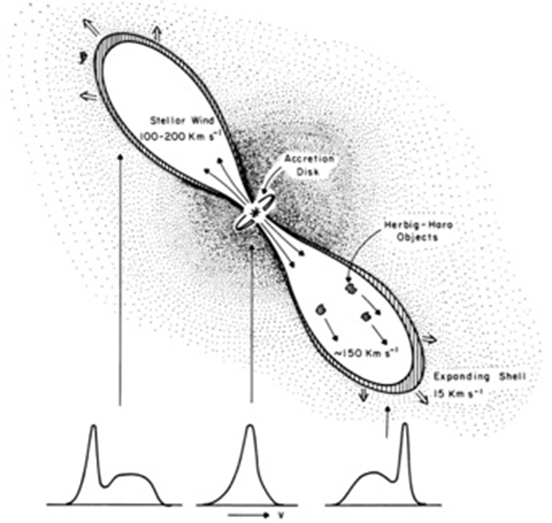
\includegraphics[width=8cm]{outflow.png}
	\caption{원시성의 방출류가 나타나는 모습으로, 아래의 스펙트럼은 왼쪽부터 red lobe, center, blue lobe의 line이다. 방출류가 나타나는 곳에서 적색/청색편이가 일어나면서 방출선의 파장이 이동된다.}
\end{figure}


\subsection{관측 대상}
\subsubsection{Orion A Cloud}

Orion Cloud에는 큰 molecular cloud들이 넓게 퍼져 있어 대부분의 별들은 $4M_{\odot}$ 이상의 질량과 1200만년 이하의 나이를 가지고 있다. 지구와의 거리는 약 450pc정도 떨어져 있다.\cite{Oriondistance} Orion Cloud는 크게 Orion A Cloud와 Orion B Cloud로 나누어지며 본 연구에서는 Orion A Cloud의 North 부근을 관측하였다. Orion A Cloud는 약 $29deg^2$의 범위를 덮고 있고, $1 \times 10^5 M_{\odot}$정도로 추정된다. OMC 1, 2, 3, OMC 1S, BN-KL Nebula 등의 hot core들이 존재한다.
Orion Molecular Cloud는 약 6000만년 전에 속도가 큰 두개의 거대 분자운들이 충돌해서 생겼다고 설명되고 있다. 그래서 적위 방향으로 큰 속도변화를 보인다. Orion A Cloud의 북쪽인 OMC 2 근처에서는 $12km/s$ 정도의 속도를 보이지만 남쪽 끝인 L1641 부근에서는 $5km/s$ 정도의 시선속도를 가지고 있다. \cite{Schulz}


\subsubsection{$\rho$ Ophiuchus Cloud}
$\rho$ Ophiuchus Cloud는 태양으로부터 가까운 별 형성 영역 중 하나로 지구로부터 약 145pc 만큼 떨어져 있다. 이는 몇 백만년 전에 생긴 성간운으로 면적은 $9.4 \deg^2$ 이다. 크게 세개의 복합체로 나눌 수 있다. 주 성간운 L1688은 많은 양의 Class 0, I, II 그리고 3인 원시성들이 존재하는 5개의 부분들로 나눠지고, 나머지 두 개의 작은 성간운은 L1689N과 L1689S으로 불린다. 본 연구에서는 L1688을 관측하였다. Ophiuchus Cloud는 강한 초신성 폭발로 만들어졌을 것이라고 예측된다. 최근 관측을 통해 많은 Stage I 원시성들이 발견되었다. 이것은 실질적인 모양을 이용해서 판별된 것이 아닌 $L_{bol}$이나 SED를 이용해서 밝혀진 것이기 때문에 실질적으로 방출류 등의 특징들을 관찰해서 이 원시성들이 Class I인지 판별해보는 것이 중요하다.\cite{Schulz}



\section{관측 데이터}

\subsection{TRAO}
대덕 전파망원경(TRAO)은 SEQUIA라는 5X5 array 수신기를 최근 개발하여 관측을 시작하였다. 이 연구에서는 이정은 교수의 TRAO key science project 중 하나의 일환으로 2017년에 관측되었던 데이터를 사용하였다. 이중 $^{13}CO$ J=1-0와 $C^{18}O$ J=1-0 관측 데이터를 사용하였다. 대덕 전파망원경은 13.7m 주경을 가지고 이 두 천이 선에서 ~45 arcsec의 공간 분해능을 가진다. 그리고 0.05 km/s의 속도 분해능으로 모두 0.4K의 잡음온도의 감도로 관측이 되었다. 이러한 TRAO로 Orion A Cloud, $\rho$ Ophiuchus Cloud를 관측한 데이터를 사용하였다.\\
$^{13}CO$와 $C^{18}O$는 $^{12}CO$에 비해 광학적으로 투명한 천이선으로 시선방향에 있는 상당부분의 물질을 추적할 수 있다. 그래서 별이 탄생하는 좁은 영역에서 매우 적은 물질로 된 방출류보다	대부분의 물질이 존재하는 외피를 추적하기에 용이하다. 본 연구에서는 TRAO 관측 데이터를 사용하여 외피의 운동학적 특성인 원시성의 속도와 선폭을 결정하고, 이를 바탕으로 다음에 기술하듯이 웹에서 받은 archive $^{12}CO$ 데이터를 사용하여 방출류의 특성을 연구하였다.

\begin{figure}[h]
	\begin{center}
		\begin{tabular}{cc}
			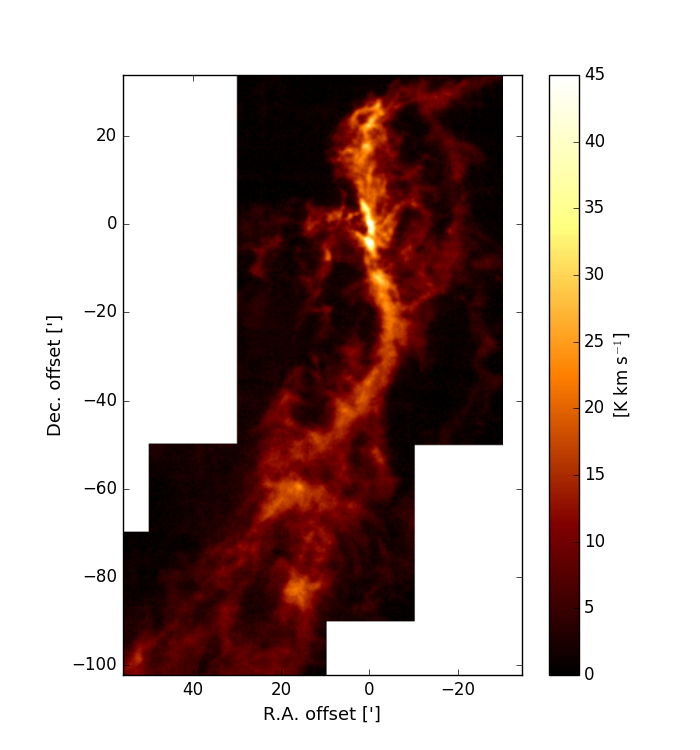
\includegraphics[height=6.5cm]{Orion_13CO_intmap.png} & 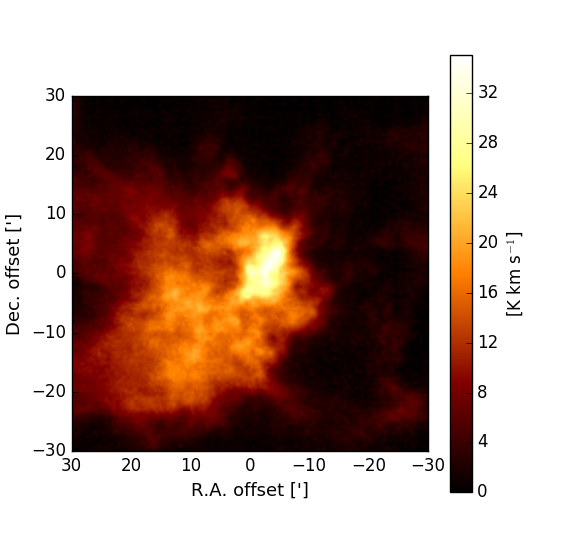
\includegraphics[height=6.5cm]{Oph_13CO_intmap.png}
		\end{tabular}
	\end{center}
	\caption{Orion A Cloud $^{13}CO$ intergrated intensity map(좌) $\rho$ Ophiuchus Cloud $^{13}CO$ intergrated intensity map(우)}
\end{figure}

\subsection{IRAM}
스페인에 있는 IRAM 30m 망원경으로 2013년에 Orion A Cloud 영역을 관측한 $^{12}CO$ J=2-1 데이터를 사용하였다. 관측데이터는 11 arcsec의 공간 분해능을 가진다. 0.4 km/s의 속도 분해능으로 0.2K의 잡음온도의 감도로 관측이 되었다.\cite{Berne}


\subsection{NRO}
일본에 있는 NRO 45m 망원경을 사용하여 2010년에 $\rho$ Ophiuchus Cloud 영역을 관측한 $^{12}CO$ J=1-0 데이터를 사용하였다. 관측데이터는 12 arcsec의 공간 분해능을 가진다. 그리고 0.4 km/s의 속도 분해능으로 0.39K의 잡음온도의 감도로 관측이 되었다.\cite{Hatchell2}
 % Introduction
	\section{Obervations and Data Reduction}

\subsection{Observation Region}
The Orion region consists of two giant molecular clouds, the Orion A and B clouds. This study covers the Orion A Cloud. The Orion A Cloud covers about $29 \, \textrm{deg}^2$ of the sky and its distance is about 450$\,$pc \cite{kounkel2017gould}. The total mass is estimated to be about $10^5 \, M_{\odot}$. It contains several hot molecular cores, such as the BN-KL nebula. It is known that the Orion Cloud was formed by a collision and fragmentation between two giant molecular clouds about 60 million years ago. The effects of the collision can be seen at the present. There is a big velocity gradient along the declination axis. On the north side of the Orion A Cloud (OMC 2) shows about 12$\, \rm km\,s^{-1}$ but on the south end (L1641) it is about 5$\, \rm km\,s^{-1}$ \cite{schulz2012formation}.

\subsection{Observation Data}
%%% 박기현 수정 시작
The $^{12}\textrm{CO (J = 2 - 1, 230.538\,GHz)}$ data was observed with the IRAM $\textrm{30\,m}$ telescope in Granada, Spain, in 2013. The spatial beamwidth was $\textrm 11^{\prime\prime}$, and the spectral resolution was 0.4$\, \rm km\,s^{-1}$. The noise level was 0.2$\, \rm K$. It only covers the north region of the Orion A cloud \cite{berne2014iram}.

The $^{12}\textrm{CO (J = 1 - 0, 115.271\,GHz})$ data was observed with the NRO 45m telescope in Nobeyama, Japan.

The $^{13}\textrm{CO (J = 1 - 0, 110.201\,GHz})$ and the $\textrm{C}^{18}\textrm{O (J = 1 - 0, 109.782\,GHz})$ data were observed with the $\textrm{13.7\,m}$ telescope at Taeduk Radio Astronomy Observatory (TRAO) in 2017. The spatial beamwidth was $\textrm 45^{\prime\prime}$, and the spectral resolution was 0.05$\, \rm km\,s^{-1}$. The noise level was 0.4$\,$K.
$^{13}\textrm{CO}$ and $\textrm{C}^{18}\textrm{O}$ lines are optically thin lines which can trace most of the matter on the line of sight, contrasting to $^{12}\textrm{CO}$ lines which are so optically oblique that it can only trace the outermost part of the molecular core. In this study, I used TRAO data to determine the protostar's velocity and linewidth which are the kinematic properties of the envelope. Then, I will trace the outflow jets using $^{12}$CO data.
%%%박기현 수정 끝

%%%선재 원본
%%%The $^{12}$CO(J = 2 - 1, $230.538\,\rm GHz$) data was observed with the IRAM 30$\,$m telescope in Granada, Spain, in 2013. The spatial beamwidth was 11", and the spectral resolution was 0.4$\, \rm km\,s^{-1}$. The noise level was 0.2$\, \rm K$. It only covers the north region of the Orion A cloud \cite{berne2014iram}. \\
%%%The $^{12}$CO (J = 1 - 0, $115.271\, \rm GHz$) data was observed with the NRO 45m telescope in Nobeyama, Japan.  \\
%%%The $^{13}$CO (J = 1 - 0, $110.201\,$GHz) and the $\textrm{C}^{18}\textrm{O}$(J = 1 - 0, 109.782 GHz) was observed at Taeduk Radio Astronomy Observatory (TRAO) 13.7$\,$m telescope in 2017. The spatial beamwidth was 45", and the spectral resolution was 0.05$\, \rm km\,s^{-1}$. The noise level was 0.4$\,$K.\\
%%%$^{13}$CO and $\textrm{C}^{18}\textrm{O}$ lines are optically thin lines which can trace most of the matter on the line of sight, contrasting to $^{12}$CO lines which are so optically oblique that it can only trace the outermost part of the molecular core. In this study, I used TRAO data to determine the protostar's velocity and linewidth which are the kinematic properties of the envelope. Then, I will trace the outflow jets using $^{12}$CO data.

Figure \ref{fig:map1} shows the data from IRAM and TRAO. The intensity of the $^{12}\textrm{CO}$ data is approximately 10 times stronger than the $^{13}\textrm{CO}$ data.

%\begin{figure}[h]
\begin{figure}[t]
	\begin{center}
		\begin{tabular}{cc}
			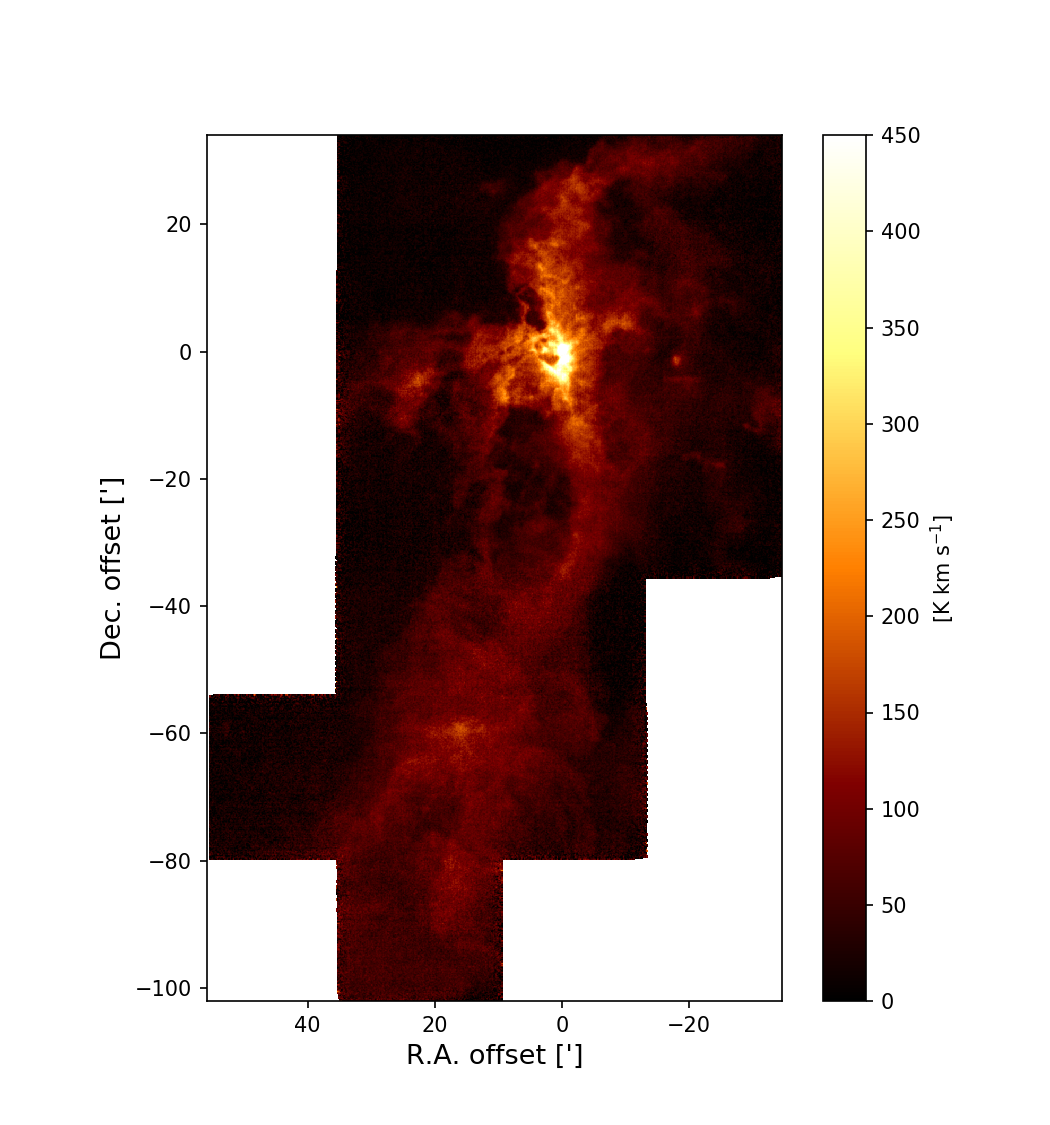
\includegraphics[width=0.45\textwidth]{RNE_12CO_Orion} & 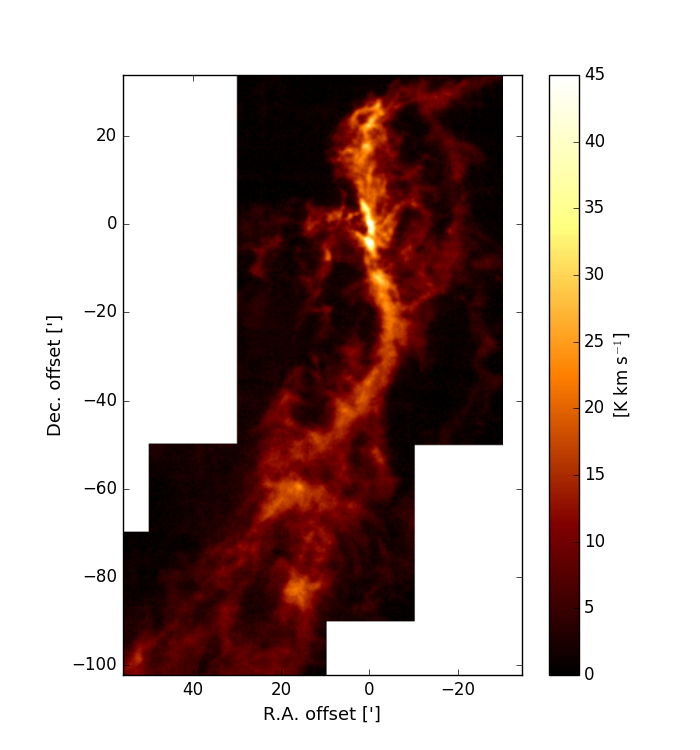
\includegraphics[width=0.45\textwidth]{Orion_13CO_intmap}
		\end{tabular}
	\end{center}
	\caption{Orion A $^{12}$CO (J = 2 - 1) integrated intensity map (left) $^{13}$CO (J = 1 - 0) integrated intensity map (right).}
	\label{fig:map1}  %%%박기현샘 추가함 (이렇게 넣어야 제데로 ref 됨.)
	%%% 박기현 레이블을 달고, 본문에서 언급하면 latex에서 알아서 같은 페이지로 보내줌.
\end{figure}

\subsection{Identification of Outflows}
Data obtained by observing radio waves were summed over the line of sight, which tells us the distribution of matter which has relative radial velocity to the observer. The envelope around the protostar is static or is contracting slowly to the protostar itself, but outflow jets have large velocity components from each pole. If the inclination of the outflows are not zero, it would be seen as jets are moving closer or further from the observer. 
In this study, $^{13}$CO and $\textrm{C}^{18}\textrm{O}$ lines were used to get the velocity distribution of the protostar. By using Gaussian fitting, I calculated the protostar’s central velocity($v_{cen}$) and the full width at half maximum (FWHM). The intervals of the red/blue lobes were defined by how far they were from the center velocity and how strong the intensity is.

Because the emission lines of $^{12}$CO are optically thicker than other lines, it is appropriate to trace the outflows with $^{12}$CO lines. I drew contour maps to find out if bipolar outflows existed with the protostar at its center. To check if the red/blue lobes that are found are outflows from the same protostar I checked the $^{12}$CO, $^{13}$CO, $\textrm{C}^{18}\textrm{O}$ lines from the red peak, blue peak, and the center points. For each outflow confirmed, I calculated the column density and the momentum force.

The column density can be calculated as the following expression:
\begin{align}
	N_{H_2} =& \frac{8\pi \nu^3}{c^3} \frac{1}{(2J_l +3)A}  \notag \\
	& \times \frac{Z(T_{ex})}{exp(-E_l / kT_{ex})[1-exp(h\nu / kT_{ex})]} \notag \\
	& \times \frac{\int T_B dV}{J(T_{ex})-J(T_{bg})} \label{column_density}
\end{align}

\begin{equation}
J(T) = \frac{h \nu / k}{exp(h\nu / kT)-1}
\end{equation}

In equation (\ref{column_density}), $\nu$ is the corresponding frequency of emission line, $c$ is the speed of light, $J_l$ is the rotational quantum number of the lower energy level, $A$ is the Einstein A coefficient, $Z$ is the partition function, $E_l$ is the rotational energy of the lower energy level, $k$ is the Boltzmann's constant, $T_{ex}$ is the excitation temperature of the transitions, $\int T_B dV$ is the integrated intensity measured, and $T_{bg}$ is the background radiation temperature. I assumed a local thermal equilibrium(LTE) excitation at an outflow temperature of 50$\,$K \cite{takahashi2008millimeter}.
The mass within one beam can be calculated as the following:

\begin{equation}
M_B =  \frac{\pi}{4} D^2 \theta_B ^2 X[\textrm{CO}] N_{\textrm{H}_2} m_{\textrm{H}_2} \label{beam_mass}
\end{equation}

$D$ is the distance to the objects, $\theta_B$ is the beam size, and $m_{\textrm{H}_2}$ is the mass of one hydrogen molecule. $X[\textrm{CO}]$ is the abundance ratio of CO to $\textrm{H}_2$. In this paper, $D = 450\,\textrm{pc}$ and $X[\textrm{CO}] = 10^{-4}$ was used \cite{hatchell2007star}.\\

\subsection{Calculating Momentum Flux}

The momentum flux within one beam is calculated as the following:

\begin{equation}
\dot{P} = \frac{dP}{dt} = \sum_{v} {\frac{M_B (v) (v/ \cos i)}{D\theta_B / (v \tan i)}}
\end{equation}

$v$ is the velocity offset from $v_{cen}$, $M_B (v)$ is the mass within one beam, and $i$ is the inclination within one beam \cite{hatchell2007star}.
Then the momentum flux from individual beams were summed in annuli. 

\begin{equation}
F_{\textrm{CO}} = \sum _{annulus} \frac{2\pi \theta_r}{N_{pix}\theta_B}\dot{P}	
\end{equation}

$N_{pix}$ is the number of pixels in a annulus. $\theta_r$ is the distance between each pixel and the outflow center. $\theta_B$ is the beam size \cite{hatchell2007star, van2013outflow}.
	
	\section{Results}


\subsection{Outflow Identification}

\begin{table}[h!]
	\caption{Protostars with observed outflows.}
	\label{table:protostars}
	\begin{center}
		\begin{tabular}{c|c|c|c|c}
			\toprule
			& \multicolumn{2}{c|}{coordinates} & $\mathbf{L_{bol}}$ & $\mathbf{T_{bol}}$\\
			\textbf{Name} & \textbf{RA} & \textbf{Dec} & $\mathbf{L_{\odot}}$ & $\mathbf{K}$\\
			\midrule
			\centering
			FIR2 & 05:35:24.3 & -05:08:33.3 & 5.68 & 100.6\\
			FIR3 & 05:35:27.5 & -05:09:32.5 & 360.86 & 71.5\\
			FIR6b & 05:35:23.4 & -05:12:03.2 & 21.93 & 54.1\\
			MMS2 & 05:35:18.3 & -05:00:34.8 & 20.11 & 186.3\\
			MMS5 & 05:35:22.4 & -05:01:14.1 & 15.81 & 42.4\\
			MMS9 & 05:35:26.0 & -05:05:42.4 & 8.91 & 38.1\\
			\midrule
		\end{tabular}
	\end{center}
\end{table}
Table \ref{table:protostars} shows the protostars with bipolar outflows observed. 

\subsubsection{$^{12}$CO J = 2 - 1 Observations}

\begin{figure}[h!]
	\begin{center}
		\begin{tabular}{cc}
			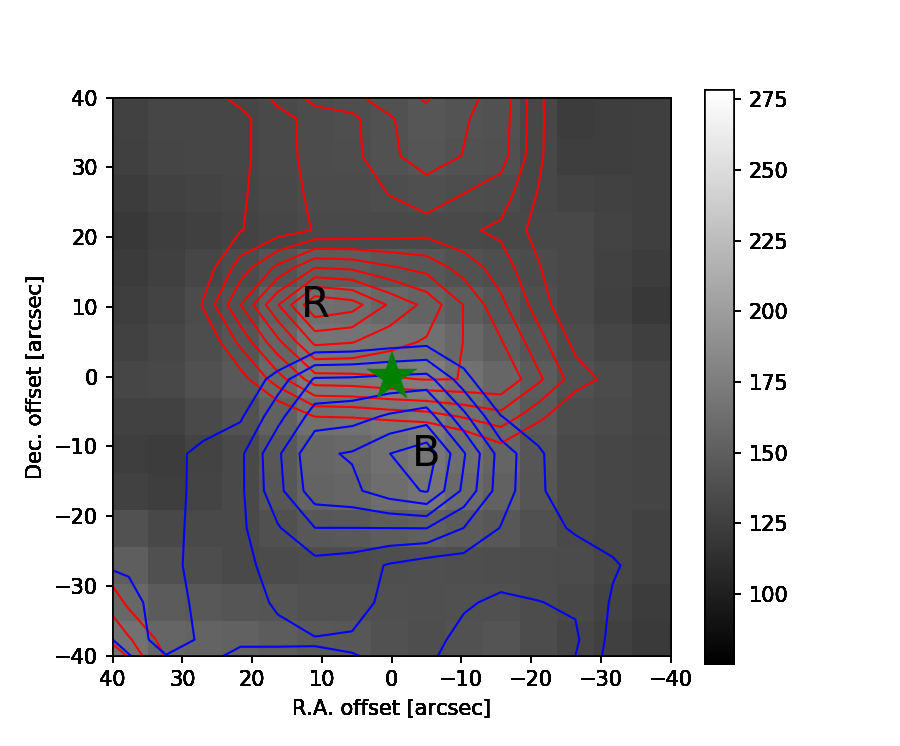
\includegraphics[width=7cm]{Orion_12CO2-1_FIR2_rbcontour_400_modified.png} &   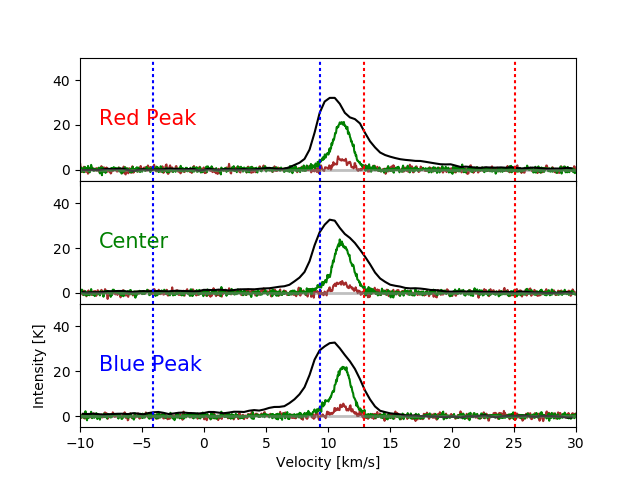
\includegraphics[width=7cm]{Orion_12CO2-1_FIR2_line_profile_400.png} \\
		\end{tabular}
		\caption{The contour map(left) and the line profile(right) of FIR2. }
		\label{fig:FIR221}
	\end{center}
\end{figure}

\begin{figure}[h!]
	\begin{center}
		\begin{tabular}{cc}
			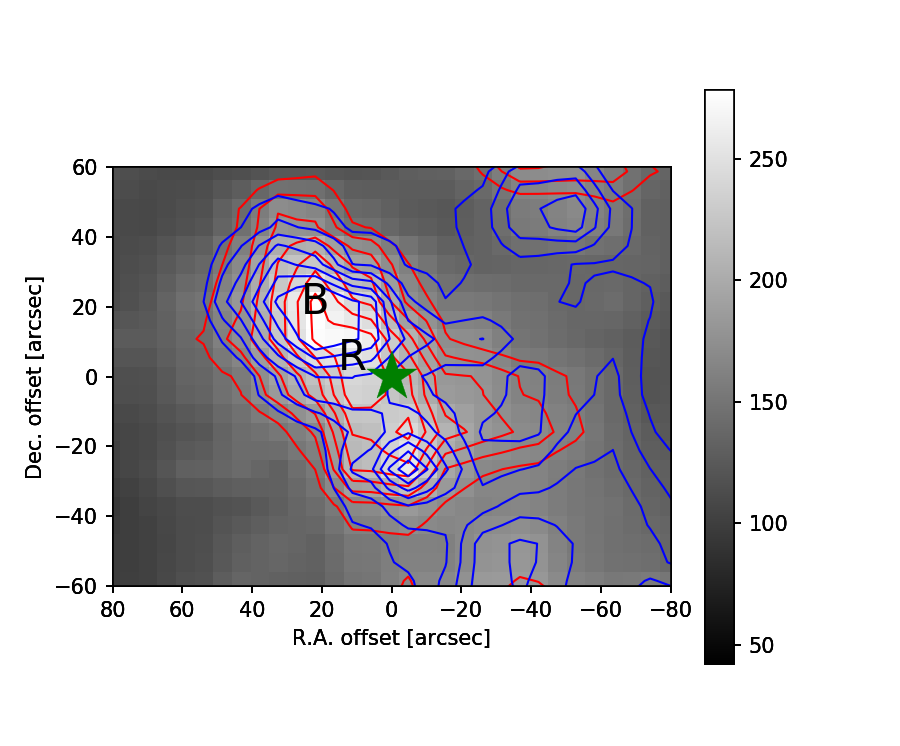
\includegraphics[width=7cm]{Orion_12CO2-1_FIR3_rbcontour_400_modified.png} &   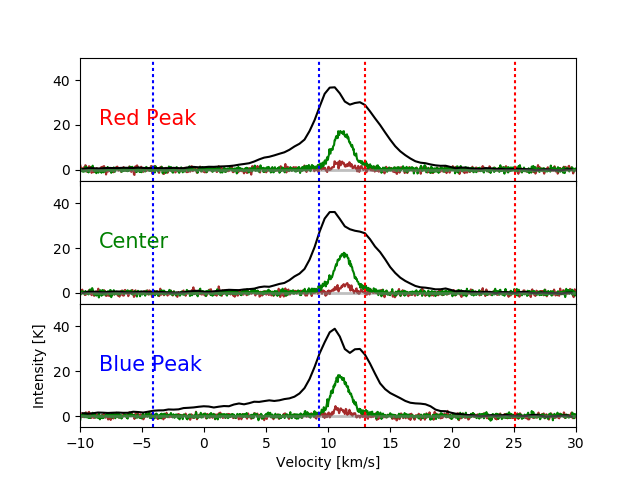
\includegraphics[width=7cm]{Orion_12CO2-1_FIR3_line_profile_400.png}\\
		\end{tabular}
		\label{FIR321}
		\caption{The contour map and the line profile of FIR3. }
	\end{center}
\end{figure}

\begin{figure}[h!]
	\begin{center}
		\begin{tabular}{cc}
			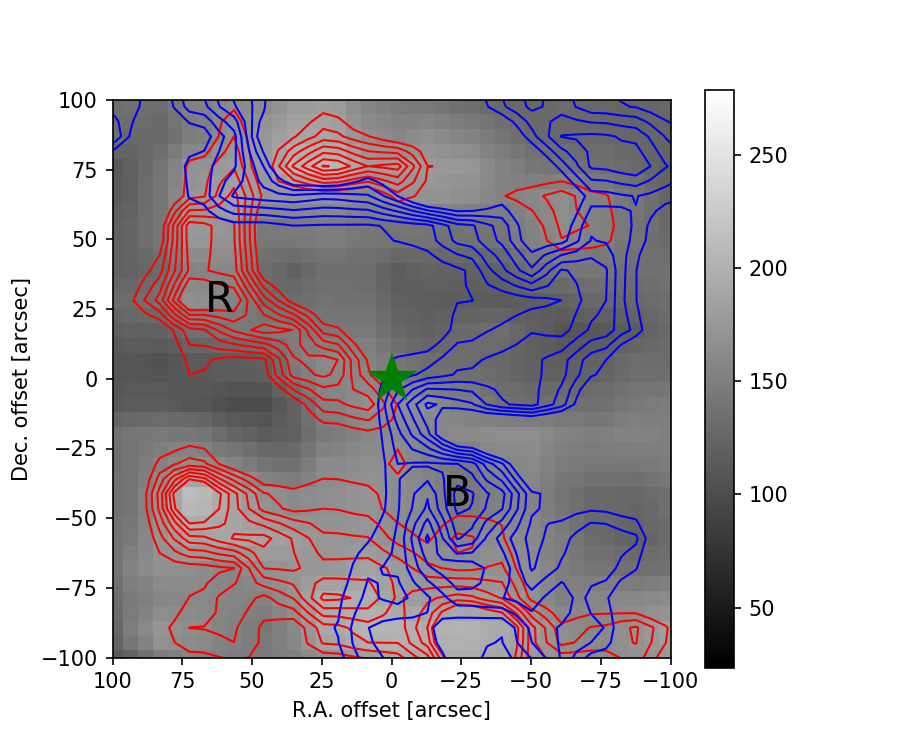
\includegraphics[width=7cm]{Orion_12CO2-1_FIR6b_rbcontour_400_modified.png} &   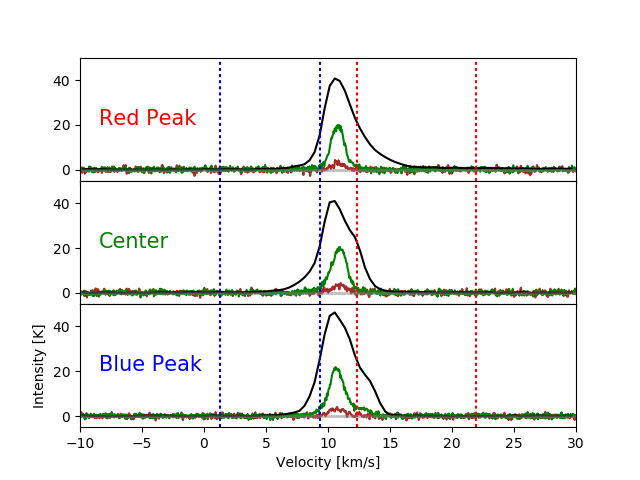
\includegraphics[width=7cm]{Orion_12CO2-1_FIR6b_line_profile_400.png}\\
		\end{tabular}
		\label{FIR6b21}
		\caption{The contour map and the line profile of FIR6b. }
	\end{center}
\end{figure}

\begin{figure}[h!]
	\begin{center}
		\begin{tabular}{cc}
			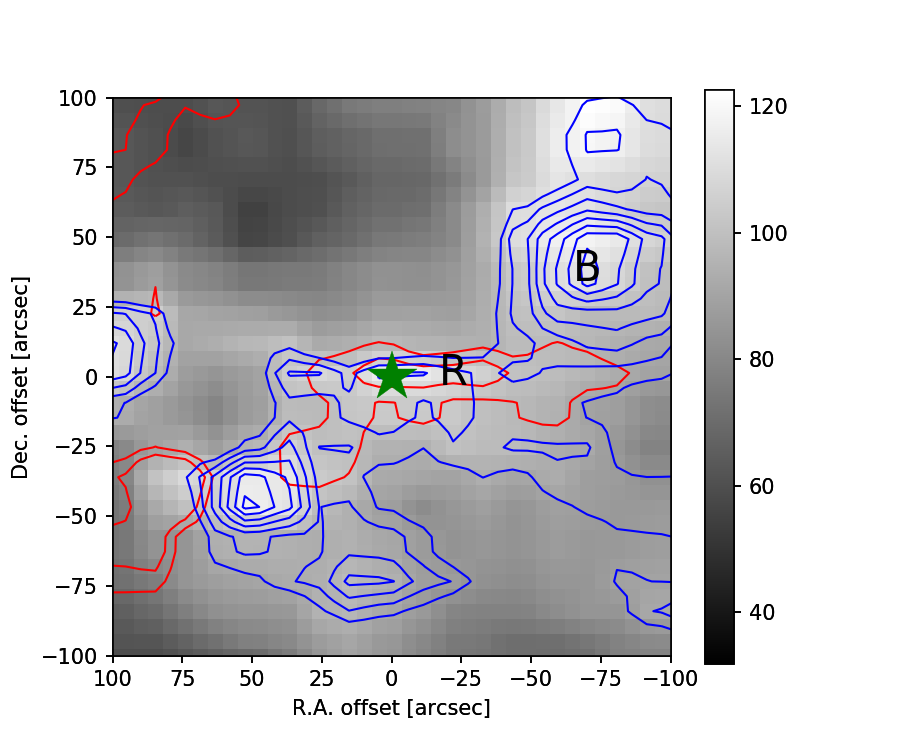
\includegraphics[width=7cm]{Orion_12CO2-1_MMS2_rbcontour_400_modified.png} &   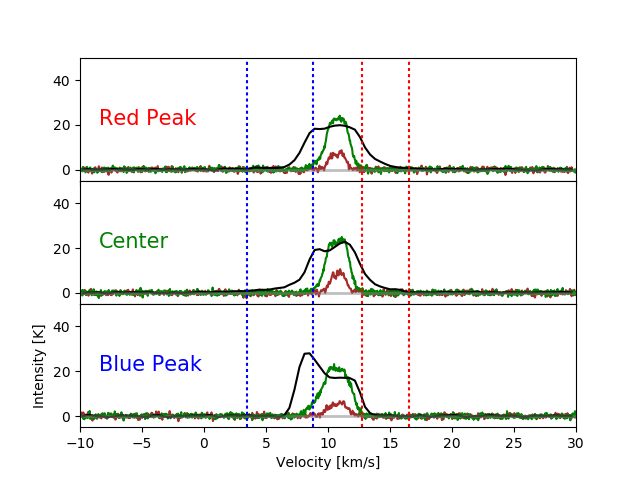
\includegraphics[width=7cm]{Orion_12CO2-1_MMS2_line_profile_400.png} \\
		\end{tabular}
		\label{MMS221}
		\caption{The contour map and the line profile of MMS2. }
	\end{center}
\end{figure}

\begin{figure}[h!]
	\begin{center}
		\begin{tabular}{cc}
			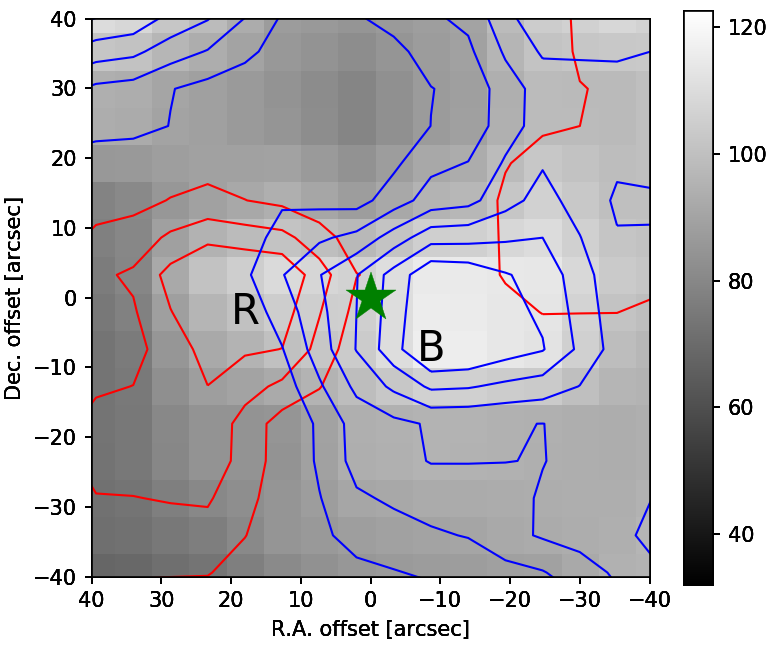
\includegraphics[width=7cm]{Orion_12CO2-1_MMS5_rbcontour_400_modified.png} &   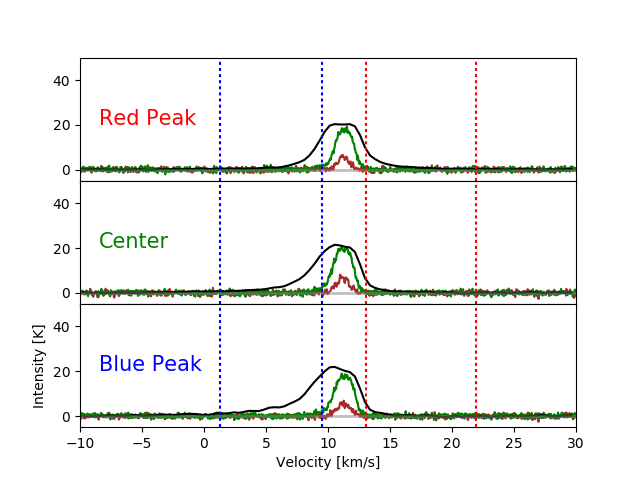
\includegraphics[width=7cm]{Orion_12CO2-1_MMS5_line_profile_400.png} \\
		\end{tabular}
		\label{MMS521}
		\caption{The contour map and the line profile of MMS5. }
	\end{center}
\end{figure}
\clearpage
\newpage
\begin{figure}[h!]
	\begin{center}
		\begin{tabular}{cc}
			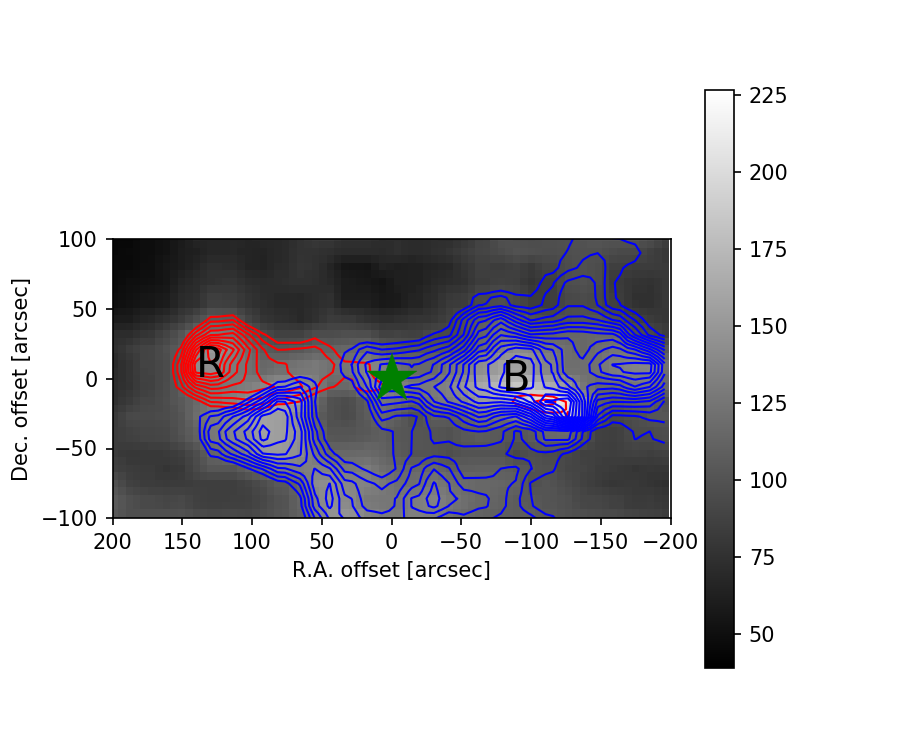
\includegraphics[width=7cm]{Orion_12CO2-1_MMS9_rbcontour_400_modified.png} &   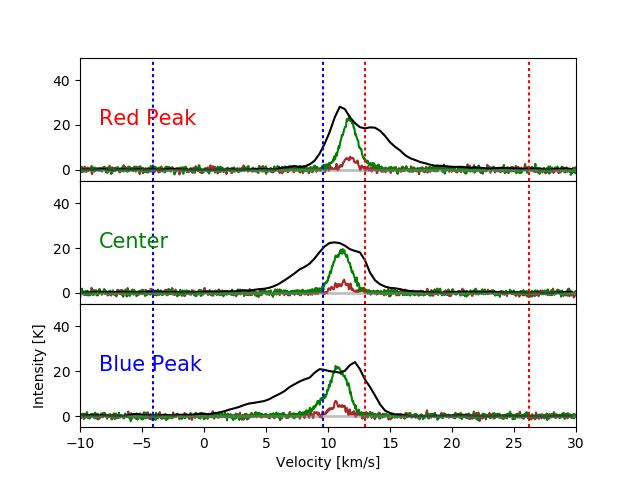
\includegraphics[width=7cm]{Orion_12CO2-1_MMS9_line_profile_400.png} \\
		\end{tabular}
		\label{MMS921}
		\caption{The contour map and the line profile of MMS9. }
	\end{center}
\end{figure}


\noindent\textbf{FIR2} - There is a strong bipolar outflow elongated along the N-S direction as shown in Figure \ref{fig:FIR221}. The size is about 30 arcsec, which is smaller than other outflows detected. Red and blue contour intervals are $10\sigma$ starting from $60\sigma$, and $10\sigma$ starting from $100\sigma$, respectively.\\
\textbf{FIR3} - A strong bipolar outflow can be seen along NE-SW direction, with red and blue lobes overlapped with each other as shown in Figure \ref{FIR321}. This tells us that the outflow axis is almost parallel to the line of sight. Red and blue contour intervals are $20\sigma$ starting from $40\sigma$, and $20\sigma$ starting from $60\sigma$, respectively. \\
\textbf{FIR6b} - The contour is not so clear because of other IR sources nearby as shown in Figure \ref{FIR6b21}. The outflow is along the NW-SE direction. Red and blue contour intervals are $10\sigma$ starting from $45\sigma$, and $10\sigma$ starting from $110\sigma$, respectively.\\
\textbf{MMS2} - The contour is in a tricky situation, because both red and blue lobes are in the east side of the protostar as shown in Figure \ref{MMS221}. The outflow structure on the SW side is the outflow from another protostar, MMS5. It is possible that the outflow structure changed shape because of the turbulence from other protostars. Red and blue contour intervals are $10\sigma$ starting from $30\sigma$, and $10\sigma$ starting from $60\sigma$, respectively.\\
\textbf{MMS5} - There is an outflow structure along the E-W direction as shown in Figure \ref{MMS521}. This outflow is much smaller than other bipolar outflows. Red and blue contour intervals are $10\sigma$ starting from $20\sigma$, and $10\sigma$ starting from $40\sigma$, respectively.\\
\textbf{MMS9} = There is a strong outflow along the E-W direction as shown in Figure \ref{MMS921}. We can see a smaller red lobe near the center of the blue lobe. Red and blue contour intervals are $10\sigma$ starting from $50\sigma$, and $10\sigma$ starting from $60\sigma$, respectively.\\

\subsubsection{$^{12}$CO J = 1 - 0 Observations}

%%%박기현 수정 시작
\begin{figure}[h!]
	\begin{tabular}{ccc}
		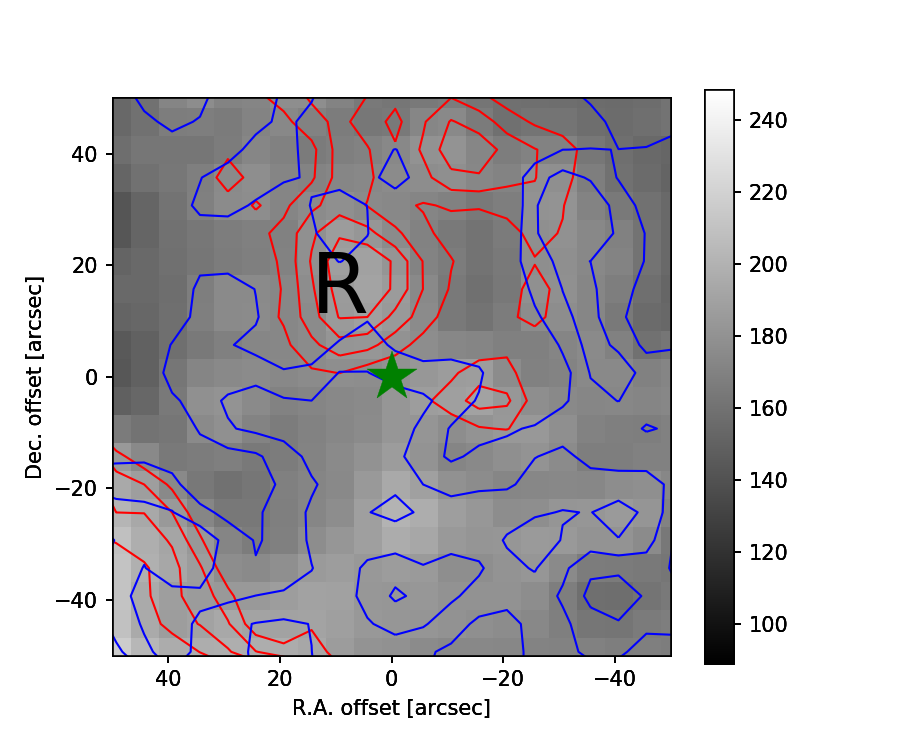
\includegraphics[width = 5cm]{Orion_12CO_NRO_HOPS68_rbcontour_400} & 
		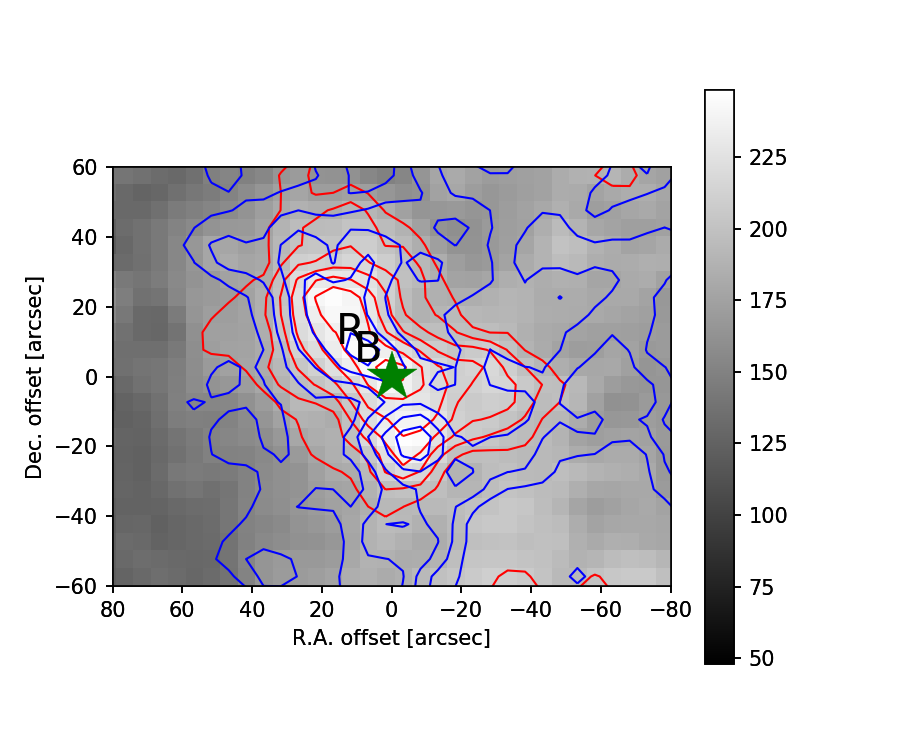
\includegraphics[width = 5cm]{Orion_12CO_NRO_HOPS370_rbcontour_400} & 
		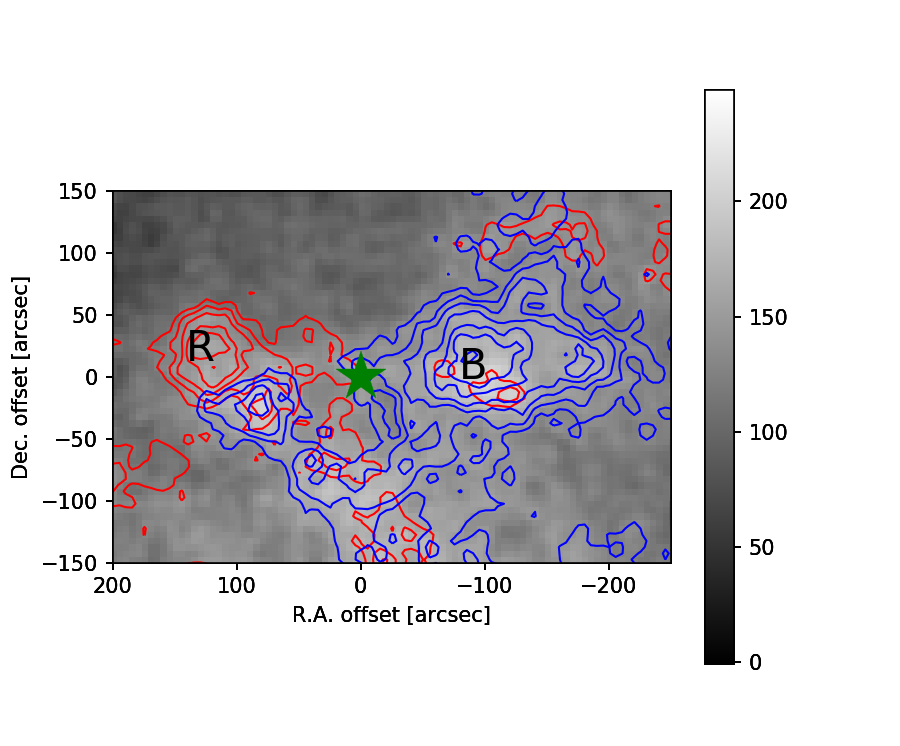
\includegraphics[width = 5cm]{Orion_12CO_NRO_HOPS78_rbcontour_400}
		\label{10}
	\end{tabular}
	\caption{The contour map of FIR2(left), FIR3(middle), and MMS9(right). }
\end{figure}
%%%박기현 수정 끝

%%%선재 원본
%%%\begin{figure}[h!]
%%%	\begin{tabular}{ccc}
%%%		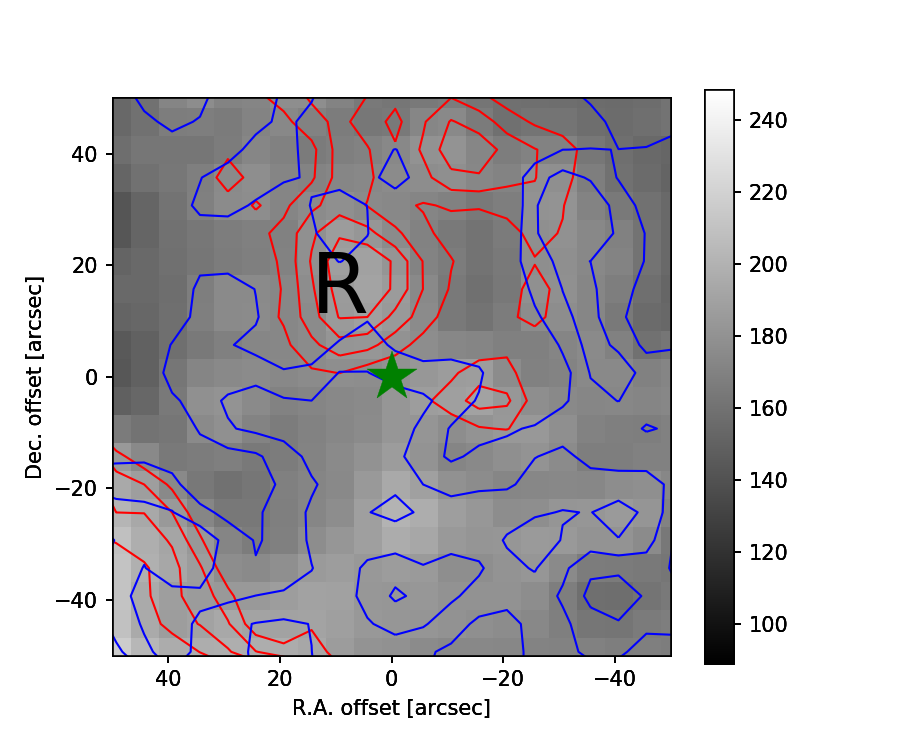
\includegraphics[width = 5cm]{Orion_12CO_NRO_HOPS68_rbcontour_400.png} & 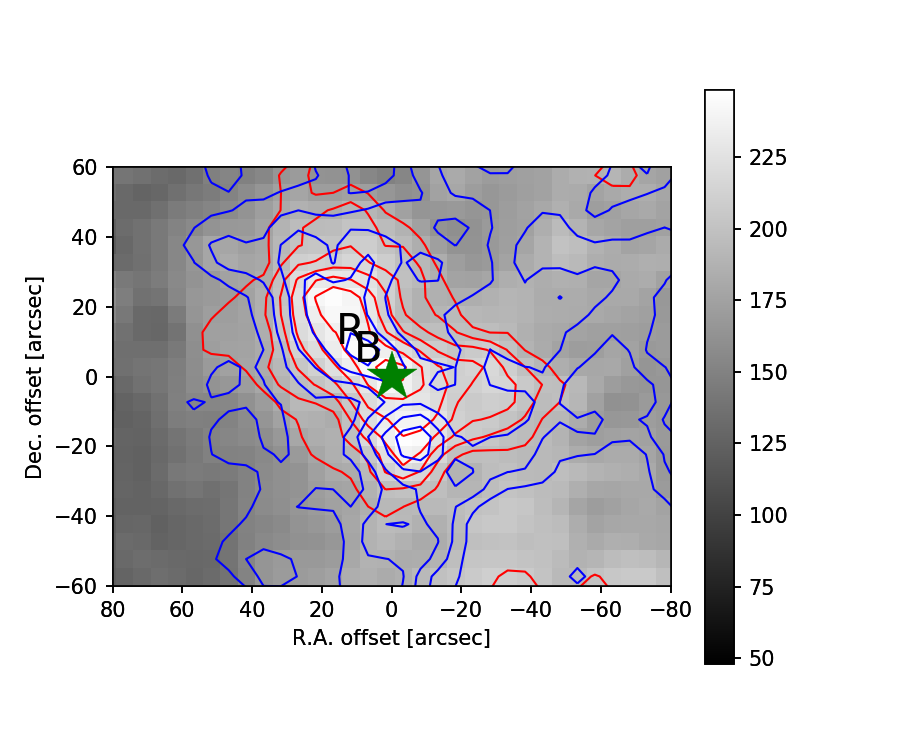
\includegraphics[width = 5cm]{Orion_12CO_NRO_HOPS370_rbcontour_400.png} & 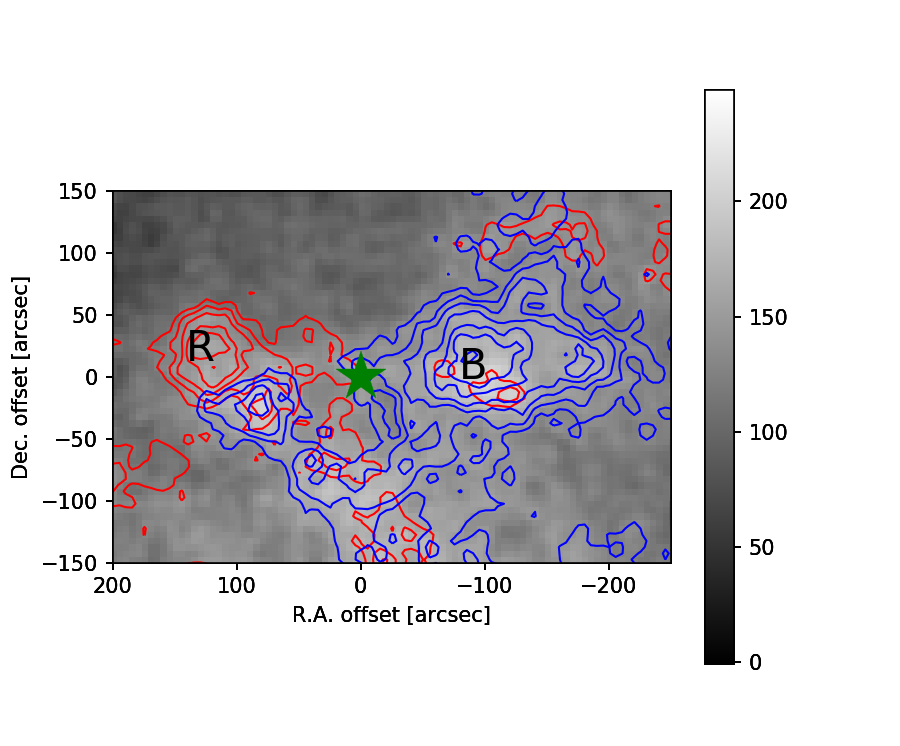
\includegraphics[width = 5cm]{Orion_12CO_NRO_HOPS78_rbcontour_400.png}
%%%		\label{10}
%%%	\end{tabular}
%%%	\caption{The contour map of FIR2(left), FIR3(middle), and MMS9(right). }
%%%\end{figure}
%%%선재 원본
 
\noindent \textbf{FIR2} - The red lobe is clear on the NW side of the protostar, but the blue lobe is not that clear as shown in Figure \ref{10}.\\
\textbf{FIR3} - The outflows are in a similar shape with the J = 2 - 1 observations as shown in Figure \ref{10}. The lobe centers are slightly near the protostar.\\
\textbf{MMS9} - The outflows are also in a similar shape with the J = 2 - 1 observations as shown in Figure \ref{10}. We can also see that there is a small red lobe near the center of the blue lobe.\\
\newpage

\subsection{Momentum Flux}


\begin{table}[h]
	\caption{CO outflow parameters.} \label{result}
	\begin{center}
		\begin{tabular}{c|c|c|c||c|c|c}
			\toprule
			\multirow{3}{1cm}{\textbf{Name}} & \multicolumn{3}{c}{J = 2 - 1} & \multicolumn{3}{c}{J = 1 - 0} \\
			& $\mathbf{F_{R}}$ & $\mathbf{F_{B}}$ & $\mathbf{F_{\textrm{\textbf{CO}}}}$ & $\mathbf{F_{R}}$ & $\mathbf{F_{B}}$ & $\mathbf{F_{\textrm{\textbf{CO}}}}$\\
			& \multicolumn{6}{c}{($M_{\odot} \, \textrm{km s}^{-1} \textrm{yr}^{-1}$)}\\
			\midrule
			FIR2 & 1.14E-05 & 3.28E-05 & 4.42E-05 & 4.78E-06 & - & 4.78E-06\\
			FIR3 & 4.77E-04 & 7.43E-04 & 1.22E-03 & 1.86E-04 & 3.02E-04 & 4.88E-04\\
			FIR6b & 1.13E-05 & 1.18E-05 & 2.31E-05 & - & - & -\\
			MMS2 & 1.14E-05 & 4.50E-05 & 5.64E-05 & - & - & -\\
			MMS5 & 5.80E-06 & 1.55E-05 & 2.13E-05 & - & - & -\\
			MMS9 & 3.67E-06 & 1.09E-05 & 1.46E-05 & 1.45E-06 & 6.02E-06 & 7.47E-06\\
			\toprule
		\end{tabular}
	\end{center}
\end{table}


Table \noindent\ref{result} shows the parameters of the outflows detected. $F_R$ and $F_B$ stands for the outflow forces for the red lobe and the blue lobe respectively. $F_{\textrm{CO}}$ is calculated by adding the two forces, which shows the momentum flux of the protostar. We can see that more outflows were detected by using J = 2 - 1 data, and the momentum flux is 2-3 times higher.\\

\clearpage
\newpage
\subsection{Momentum flux vs. Bolometric luminosity}


\begin{figure}[h!]
	\centering
	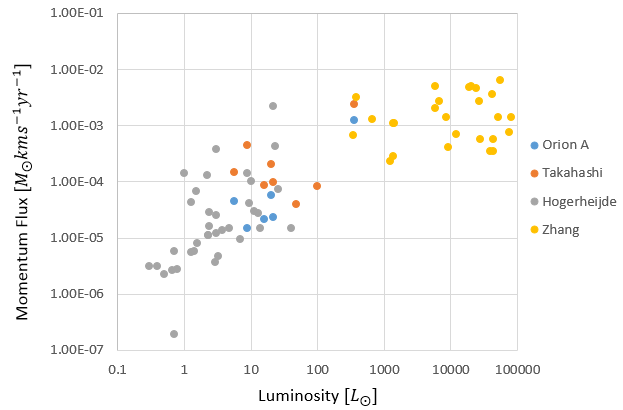
\includegraphics[width=0.95\textwidth]{Luminosity}
	\caption{Momentum flux difference by emission line energy.}
	\label{fig:lum}
\end{figure}


Figure \ref{fig:lum} shows the relation between the bolometric luminosity and the momentum flux of the outflows from previous studies \cite{takahashi2008millimeter, van2013outflow, hogerheijde1998envelope, nakamura2012evidence, aso2000dense, zhang2005search}. \\ Since the momentum flux of the same protostar is known to vary somewhat depending on the calculation methods\cite{van2013outflow}, the relation between the bolometric luminosity and the momentum flux is difficult to express with the excat formula and only the degree of tendency can be analyzed.
The bolometric luminosity was observed by the Spitzer and Herschel telescopes. Orion A Cloud is a region where stars with medium mass are formed. The fact that the momentum flux of the outflow is proportional to the bolometric luminosity could be checked.

\newpage

\subsection{Momentum flux by emission line energy level}

\begin{figure}[h!]
	\centering
	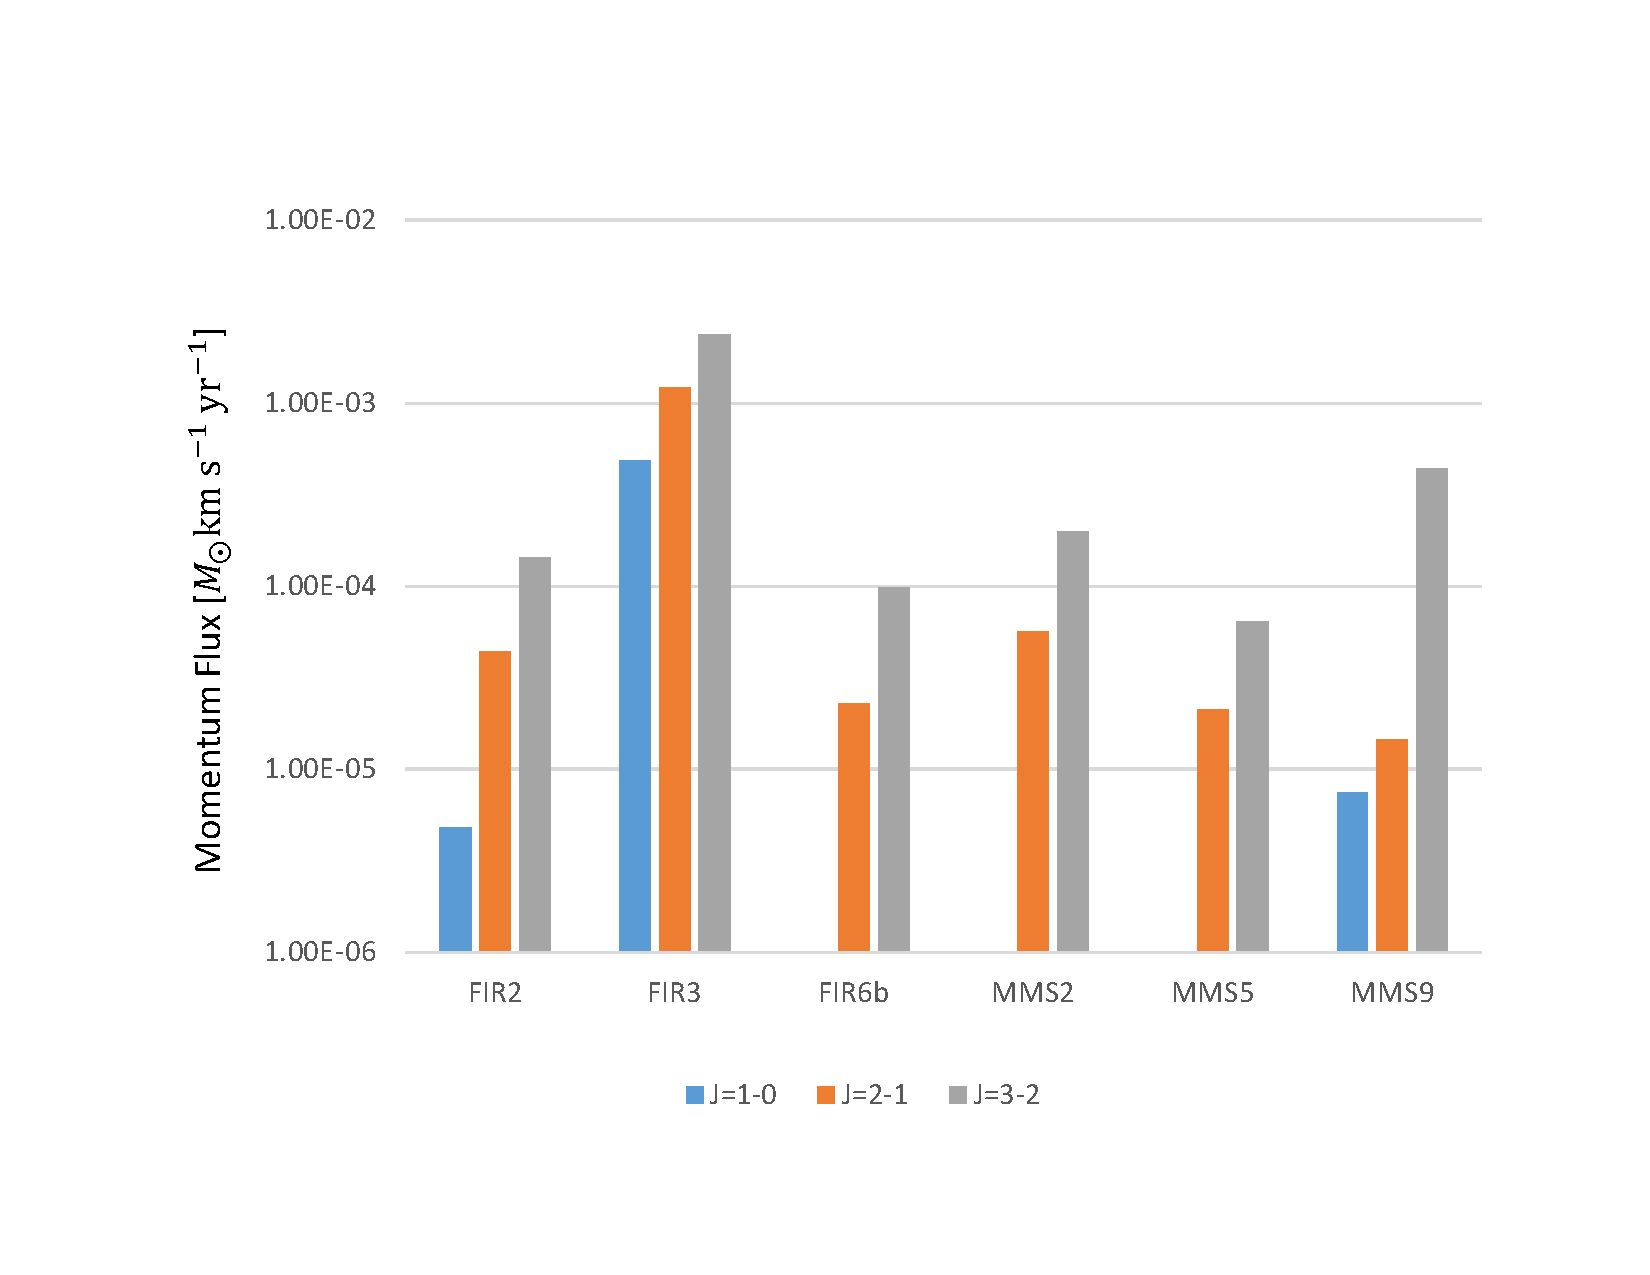
\includegraphics[width=\textwidth]{outflow_J}
	\ref{J}
	\caption{Momentum flux difference by emission line energy.}
\end{figure}

Figure \ref{J} compares momentum flux calculated by three different emission lines of the same protostar. The $^{12}$CO J = 3 - 2 observation was made by Takahashi et al \cite{takahashi2008millimeter}. We can see that it is possible to detect more outflows by using a higher energy emission line of $^{12}$CO. Using data with smaller beamwidth also enhances detecting outflows. The reason that higher energy lines can detect more outflows can be explained as the following. The excitation temperature is higher for emission lines with higher energy. Outflows drag out matter from the protostar's envelope, which has higher temperature than its surroundings. Lines with higher energy are emitted, which has an effect that makes column density higher than usual.
	%-----------------------------------------------------
% Conclusion
%-----------------------------------------------------
\newpage

\section{Conclusion}
The main results of this study are as follows:
\begin{enumerate}
	\item 6 bipolar outflows were detected from the Orion A Cloud. All outflows were detected by J = 2 - 1 data and 3 outflows were detected by J = 1 - 0 data.
	\item The well-known correlation between the momentum flux and the bolometric luminosity can be checked.
	\item It is possible to detect more outflows by using a higher energy emission line of $^{12}$CO. Using data with smaller beamwidth also enhances detecting outflows. The reason that higher energy lines can detect more outflows can be explained as the following. The excitation temperature is higher for emission lines with higher energy. Outflows drag out matter from the protostar's envelope, which has higher temperature than its surroundings. Lines with higher energy are emitted, which has an effect that makes column density higher than usual.	
\end{enumerate} % Conclusion
	
	%%\clearpage  %%% Appendix를 새 페이지에서 시작
\appendix
\renewcommand{\thesection}{\Alph{section}} %%% TOC에 appendix numbering 재설정
\renewcommand{\thesubsection}{\arabic{subsection}}
\renewcommand{\thesubsubsection}{\arabic{subsubsection}}
\titleformat{\section}[hang] {\normalfont\fontsize{21}{21}\selectfont\bfseries}{\Alph{section}.}{1em}{} %%% Appendix section title의 재설정
\titleformat{\subsection}[hang] {\normalfont\fontsize{16}{16}\selectfont\bfseries}{\Alph{section}.\arabic{subsection}.}{1em}{}
\titleformat{\subsubsection}[hang] {\normalfont\fontsize{14}{14}\selectfont}{\Alph{section}.\arabic{subsection}.\arabic{subsubsection}.}{1em}{}
\titleformat{\paragraph}[hang] {\normalfont\fontsize{12}{12}\selectfont\it}{}{1em}{}
\renewcommand{\theequation}{\thesection.\arabic{equation}} %%% Appendix equation numbering 의 재설정
\renewcommand{\thefigure}{\thesection-\arabic{figure}} %%% Appendix figure numbering 의 재설정
\renewcommand{\thetable}{\thesection-\arabic{table}} %%% Appendix table numbering 의 재설정
\setcounter{equation}{0} %%% Appendix equation starting number의 초기화
\setcounter{figure}{0} %%% Appendix figure starting number의 초기화
\setcounter{table}{0} %%% Appendix table starting number의 초기화
\section{부록}
\begin{table}[h!]
	\begin{center}
		\begin{tabular}{c|c|c|c|c|c|c|c|c}
			\toprule
			&\multicolumn{4}{c|}{Previous Work} & \multicolumn{4}{c}{Our Work}\\
			&\multicolumn{2}{c|}{Blue Lobe} & \multicolumn{2}{c|}{Red Lobe} & \multicolumn{2}{c|}{Blue Lobe} & \multicolumn{2}{c}{Red Lobe}\\
			\textbf{Name} & $\mathbf{v_{out}}$ & $\mathbf{v_{in}}$ & $\mathbf{v_{out}}$ & $\mathbf{v_{in}}$&$\mathbf{v_{out}}$ & $\mathbf{v_{in}}$ & $\mathbf{v_{out}}$ & $\mathbf{v_{in}}$\\
			& [km/s] & [km/s] & [km/s] & [km/s] & [km/s] & [km/s] & [km/s] & [km/s] \\ 
			\midrule
			\multicolumn{9}{c}{Orion A Cloud}\\
			\midrule
			FIR2 & -4.1 & 8.9 & 13.2 & 20.8 &-4.1 & 9.4 & 12.9 & 20.8\\
			FIR3 & -4.1 & 8.9 & 13.2 & 25.1 & -4.1 & 9.25 & 13.0 & 25.1\\
			FIR6b & 1.3 & 8.9 & 13.2 & 21.9 & 1.3 & 9.3 & 12.4 & 21.9\\
			MMS2 & 3.5 & 8.9 & 13.2 & 16.5 & 3.5 & 8.8 & 12.8 & 16.5\\
			MMS5 & 1.3 & 8.9 & 13.2 & 21.9 & 1.3 & 9.5 & 13.1 & 21.9\\
			MMS9 & -4.1 & 8.9 & 13.2 & 26.2 & -4.1 & 9.6 & 13.0 & 26.2\\
			\midrule
			\multicolumn{9}{c}{$\rho$ Ophiuchus Cloud}\\
			\midrule
			Elias 32 & -6.7 & 0.8 & 6.0 & 10.3 & -6.7 & 1.2 & 5.3 & 10.3\\
			IRS 46 & -3.7 & 0.4 & 6.5 & 14.1 & -1.2 & 1.1 & 5.9 & 8.4\\
			VLA 1623 & -3 & 10 & 6.5 & 13 & -3 & 1.2 & 5.3 & 9\\
			BBRCG 24 & N.A. & N.A. & N.A. & N.A. & -5 & 1.2 & 5.7 & 9\\
		\end{tabular}
	\end{center}
	\caption{관측한 원시성들의 적색/청색편이 속도 구간}
\end{table} % Appendix가 없는 경우 주석처리하십시오
	
	\bibliography{bibfile} % 참고문헌
	% BibTeX 코드 쉽게 얻어오는 방법 %
	% Google Scholar 에서 검색한 결과에서 `인용'을 클릭한다.
	% BibTeX 코드를 얻고자 한다면, 하단의 `BibTeX' 을 클릭.
	% 코드가 나온다. Ctrl+A, Ctrl+C로 복사, bibfile에 붙여넣기.
	
	%\begin{summary}
\addcontentsline{toc}{section}{Summary}  %%% TOC에 표시
한글로 졸업논문을 작성한 학생은 반드시 5페이지 내외의 영어 요약문을 작성해야 합니다. 영문으로 작성하는 학생은 이 부분을 작성하지 않아도 됩니다.
\end{summary} % Summary
	%(영어로 작성한 학생은 이 부분을 주석 처리하십시오.)
	
	%-----------------------------------------------------
%   감사의 글
%-----------------------------------------------------
\begin{acknowledgements}
\addcontentsline{toc}{section}{감사의 글}  %%% TOC에 표시
정말 감사합니다.
\end{acknowledgements}

%-----------------------------------------------------
%   연구활동 
%-----------------------------------------------------
\begin{researches}
\addcontentsline{toc}{section}{연구활동}  %%% TOC에 표시
\begin{itemize}
\item{2011학년도 교내 R\&E 발표대회에서 장려상 수상}
\item{2012학년도 교내 R\&E 발표대회에서 장려상 수상}
\item{2013학년도 교내 R\&E 발표대회에서 장려상 수상}
\item{2014학년도 교내 R\&E 발표대회에서 장려상 수상}
\item{2015학년도 교내 R\&E 발표대회에서 장려상 수상}
\item{2016학년도 교내 R\&E 발표대회에서 장려상 수상}
\item{2017학년도 교내 R\&E 발표대회에서 장려상 수상}
\item{2018학년도 교내 R\&E 발표대회에서 장려상 수상}
\item{2019년 노벨 물리학상 수상}
\end{itemize}
\end{researches} % 감사의 글 & 연구활동
\end{document}